% !TeX encoding = ISO-8859-1
% !TeX spellcheck = fr_FR
% !TeX root = syllabus_ELEC0053.tex

\chapter{Méthodes matricielles  d'analyse et\\ de représentation des circuits}
\label{sec:methodes-generales}

\textit{La mise en équation de circuits sous forme matricielle et les méthodes de résolution correspondantes ont plusieurs utilités. Premièrement, elles permettent de systématiser l'approche d'analyse d'un circuit. Deuxièmement, par des manipulations matricielles, elles permettent de représenter un circuit via un équivalent de Thévenin ou de Norton, mais à plus d'un accès. Ceci est particulièrement intéressant, par exemple, si on souhaite réduire un circuit à un quadripôle. Finalement, cela ouvre la porte à la résolution numérique de circuits.
L'analyse présentée dans ce chapitre se limite à une représentation  en courant continu. Les méthodes sont cependant directement extensibles au cas du régime sinusoïdal avec l'emploi des phaseurs, et même à l'analyse transitoire en utilisant la représentation dans le domaine de Laplace, mais ce dernier point est hors du cadre de ce cours. }

\section{La méthode des noeuds}

Les variables considérées dans cette méthode sont les variables relatives aux noeuds du réseau : potentiel de chacun des noeuds par rapport à celui de référence, et courants de noeuds, ceux-ci étant précisés ultérieurement.

\subsection{Vue générale de la méthode}
Pour déterminer l'état électrique d'un système, la méthode des noeuds consiste à résoudre le système linéaire suivant : 
$$\mathbf{G}_N \mathbf{v}_N = \mathbf{i}_{sN}.$$
où 
\begin{itemize}
\item L'indice $N$ signifie "Noeud".
\item $\mathbf{i}_{sN}$ est le vecteur des injections de courant aux noeuds. Déterminé par inspection, il caractérise l'impact des sources indépendantes de courant.
\item $\mathbf{v}_N$ est le vecteur des potentiels de noeuds. Il contient les $n-1$ variables du système (tous les noeuds sauf un noeud de référence), et les courants de branches en découlent, via la loi d'Ohm.
\item $\mathbf{G}_N$ est la matrice de conductances aux noeuds. Déterminée par inspection ou par expérimentation, elle caractérise le graphe du circuit passifié.
\end{itemize}

Algorithmiquement, la méthode se résume aux cinq étapes principales décrites dans la Table~\ref{tab:methode_noeuds}.
\begin{table}[tb]
	\caption{Vue algorithmique de la méthode des noeuds. \label{tab:methode_noeuds}}
	\begin{boxedminipage}{\textwidth}
	\begin{enumerate}
	\item Choisir un noeud de référence,
	\item déterminer la matrice $\mathbf{G}_N$,
	\item déterminer le vecteur $\mathbf{i}_{sN}$,
	\item résoudre le système $$\mathbf{G}_N \mathbf{v}_N = \mathbf{i}_{sN}$$ pour obtenir les potentiels de noeuds,
	\item déduire de $\mathbf{v}_N$ les courants dans les branches.
	\end{enumerate}
	\end{boxedminipage}
\end{table}
Cette méthode est applicable si le circuit est linéaire et s'il ne comporte que des sources indépendantes de courant\footnote{ Nous verrons plus tard comment gérer les sources indépendantes de tension et les source commandées de courant (VCT).}.

\subsection{Dérivation de la méthode des noeuds}

Les trois relations suivantes, reposant sur la matrice d'incidence et la matrice de conductance, traduisent respectivement la PLK (\ref{eq:MN_1}), le lien entre tension de branche et potentiel de noeud (\ref{eq:MN_2}), et la loi d'Ohm (\ref{eq:MN_3}) :
\begin{align}
\mathbf{A} \mathbf{i}_B &= \mathbf{i}_{sN} \label{eq:MN_1}\\
\mathbf{u}_B &= \mathbf{A}^T \mathbf{v}_{N} \label{eq:MN_2}\\
\mathbf{i}_B &= \mathbf{G}_B \mathbf{u}_{B} \label{eq:MN_3}
\end{align}
On établit ensuite le système résolu par la méthode des noeuds sur base de ces trois relations par simples manipulations et en définissant la \textit{matrice de conductance aux noeuds} $\mathbf{G}_N.$
\begin{align}
(\ref{eq:MN_3}) \rightarrow (\ref{eq:MN_1}) \quad \mathbf{A} \mathbf{G}_B \mathbf{u}_{B} &= \mathbf{i}_{sN} \label{eq:MN_4}\\
(\ref{eq:MN_2}) \rightarrow (\ref{eq:MN_4}) \quad \mathbf{A} \mathbf{G}_B \mathbf{A}^T \mathbf{v}_{N} &= \mathbf{i}_{sN} \label{eq:MN_5}\\
\mathbf{G}_N &\triangleq \mathbf{A} \mathbf{G}_B \mathbf{A}^T \label{eq:MN_6}\\
(\ref{eq:MN_6}) \rightarrow (\ref{eq:MN_5}) \quad \mathbf{G}_N &\mathbf{v}_N = \mathbf{i}_{sN}
\end{align}

\subsection{Matrice d'incidence}
Les relations de base sont les expressions faisant intervenir la matrice d'incidence réduite, définie ci-dessous.


Nous considérons un graphe orienté à $n$ noeuds et $b$ branches
et définissons des matrices décrivant les relations d'appartenance noeuds-branches\footnote{Dans la méthodes des mailles (Section~\ref{sec:MM}), nous nous intéresserons à la relation branches-mailles.}.
Un intérêt tout particulier est réservé à la recherche de matrices qui contiennent le nombre nécessaire et
suffisant de relations, c'est-à-dire à la détermination du rang de chacune de ces matrices.

\paragraph{Matrice d'incidence complète $\mathbf{A}_a$.} C'est une matrice d'ordre $n \times b$ où chaque élément $a_{ij}$ est défini comme suit:
\begin{enumerate}
\item $a_{ij} = -1$ si la branche $j$ est incidente au noeud $i$ et est orientée vers lui ;
\item $a_{ij} = +1$ si la branche $j$ est incidente au noeud $i$ et est orientée en sens opposé ;
\item $a_{ij} = 0$ si la branche $j$ n'est pas incidente au noeud $i$
\end{enumerate}

Par construction, chaque ligne de $\mathbf{A}_a$ correspond ainsi à un noeud, ses éléments non
nuls identifiant les branches incidentes à celui-ci. De même, chaque colonne correspond
à une branche. Elle comporte donc nécessairement deux éléments non nuls, un $+1$ et
un $- 1$ , dont la somme est évidemment nulle. Cette dernière observation conduit à la conclusion que $\mathbf{A}_a$ comporte un nombre
surabondant de relations et que le rang de $\mathbf{A}_a$ est inférieur à $n$.

\begin{testexample}[Matrice d'incidence.]
Soit le réseau ci-dessous et sa représentation sous forme de graphe orienté (à droite).
\begin{center}
\centering
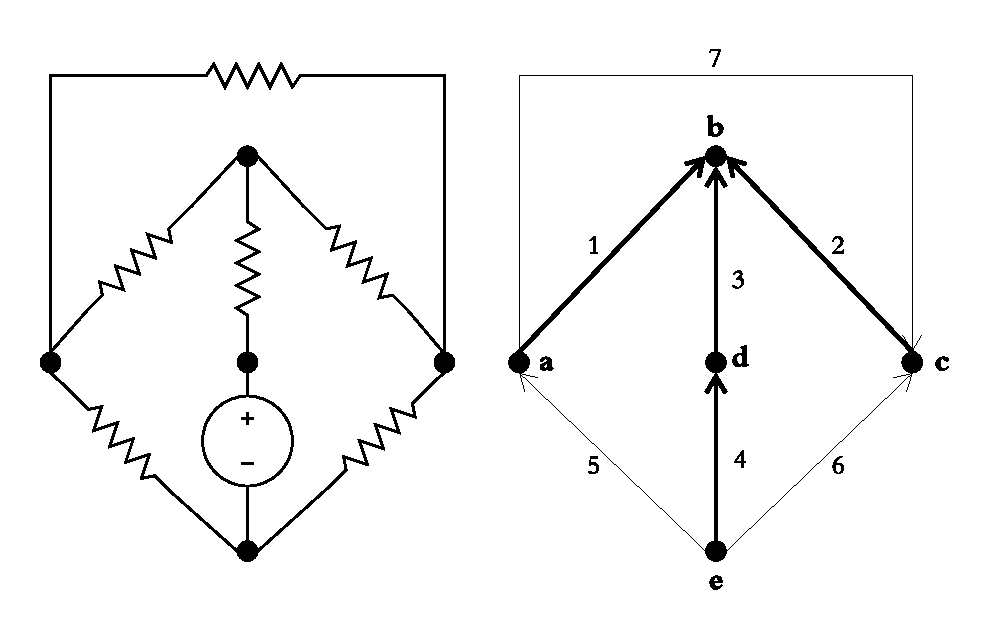
\includegraphics[width=0.9\linewidth]{figs/graphes/circuit_et_graphe}
\end{center}
Il comporte $n=5$ noeuds. La PLK en chacun des noeuds s'écrit
$${\small 
\begin{array}{rccccccccccccccccl}
	a & : &  &i_1&  &   &  &   &  &   & - & i_5 & &   & + & i_7 & = & 0\\ 
	b & : & -&i_1& -&i_2&- &i_3&  &   &   &     & &   &   &     & = & 0\\
	c & : &  &   &  &i_2&  &   &  &   &   &     &-&i_6& - & i_7 & = & 0\\
	d & : &  &   &  &   &  &i_3&- &i_4&   &     & &   &   &     & = & 0\\
	e & : &  &   &  &   &  &   &  &i_4& + & i_5 &+&i_6&   &     & = & 0
\end{array}}
$$
Ce qui conduit à la matrice d'incidence
$$\mathbf{A}_a = \left[\begin{array}{rrrrrrr}
	1 & 0 & 0 & 0 & -1 & 0 & 1\\
	-1&-1 & -1& 0 & 0  & 0 & 0\\
	0 & 1 & 0 & 0 & 0  &-1 &-1\\
	0 & 0 & 1 &-1 & 0 & 0 & 0\\
	0 & 0 & 0 & 1 & 1 & 1 &0
\end{array}\right]$$
On voit directement que la dernière ligne est l'opposé de la somme des quatres premières.
\end{testexample}



\paragraph{Matrice d'incidence (réduite) $\mathbf{A}$.}
En choisissant un noeud de référence puis en éliminant la relation liée à ce noeud, on obtient la  matrice $\mathbf{A}$ issue de $\mathbf{A}_a$ et d'ordre $(n-1) \times b$. On peut montrer que cette matrice est de rang $n-1$, en tous les cas si le graphe est connexe.
  
\begin{testexample}[Matrice d'incidence réduite.]
Dans l'exemple précédent, choisissons le noeud $e$ comme noeud de référence. Cela implique que l'on supprime la relation liée à ce noeud, et que $e$ sera considéré comme référentiel de tension, c'est-à-dire que $v_e = 0$. Le rang de cette matrice est $n-1$.
\[ {\bf A} = 
\left[\begin{array}{rrrrrrr}
1 & 0 & 0 & 0 & -1 & 0 & 1\\
-1&-1 & -1& 0 & 0  & 0 & 0\\
0 & 1 & 0 & 0 & 0  &-1 &-1\\
0 & 0 & 1 &-1 & 0 & 0 & 0
\end{array}\right] \]
Le rang de la matrice est $4$.
\end{testexample}
On peut maintenant écrire $${\bf A}\, {\bf i}_B =  {\bf 0},$$
avec $n-1$ relations linéairement indépendantes, où
${\bf i}_B$ est le vecteur des courants de branches orientés selon le sens que l'on a choisi pour construire ${\bf A}$.

\subsection{Vecteur d'injections de courant} Nous avons jusqu'à présent considéré le graphe passifié. Considérons maintenant l'impact des sources indépendantes de courant à travers le vecteur ${\bf i}_{sN}$ de taille $n-1$ qui caractérise les courants injectés aux différents noeuds (sauf le noeud de référence) par les sources indépendantes. Une injection est prise avec le signe "$+$" si le courant est orienté vers le noeud, "$-$" sinon.

\begin{testexample}[Vecteur $\mathbf{i}_{sN}$.]
Soit le circuit suivant, où le noeud $d$ est pris comme référence.
\begin{center}
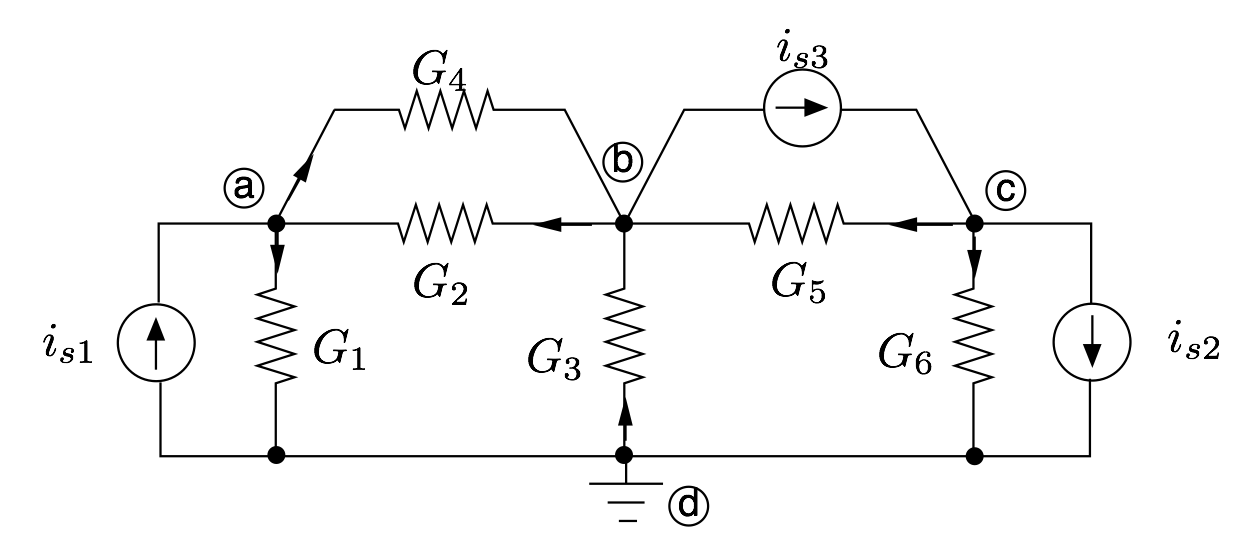
\includegraphics[width=0.8\linewidth]{figs/methodes-generales/exemple_iSN}
\end{center}
On a 
\[ {\bf i}_{sN} = 
\left[
\begin{array}{c}
i_{s1}\\
-i_{s3}\\
i_{s3}-i_{s2}
\end{array} \right] \]
\end{testexample}
Avec ces conventions, on a 
$${\bf A}\, {\bf i}_B =  {\bf i}_{sN}.$$

\subsection{Tensions de branches}
Par définition, la matrice d'incidence caractérise également la relation entre potentiels de noeuds et tension de branche (d.d.p. entre les extrémités d'une branche) : 
$$\mathbf{u}_B = \mathbf{A}^T \mathbf{v}_{N}.$$
La convention moteur est utilisée, selon le sens qui a été choisi pour orienter (le courant dans) les branches.

\begin{testexample}
Soit le graphe suivant : 
\begin{center}
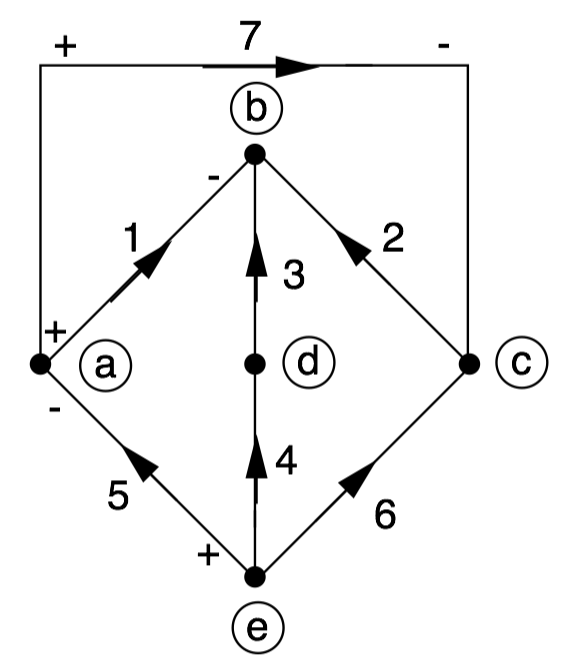
\includegraphics[width=0.4\linewidth]{figs/methodes-generales/exemple_tension_branche}
\end{center}
Le noeud $e$ étant pris comme référence, on a 
{\small $$
\left[\begin{array}{c}
u_1 \\
u_2 \\
u_3 \\
u_4 \\
u_5 \\
u_6 \\
u_7 
\end{array}\right] = 
\left[\begin{array}{rrrr}
1 & -1 & 0 & 0\\
0 & -1 & 1 & 0\\
0 & -1 & 0 & 1\\
0 & 0 & 0 & -1\\
-1 & 0 & 0 & 0 \\
0 & 0 & -1 & 0 \\
1 & 0 & -1 & 0
\end{array}\right]
\left[\begin{array}{c}
v_a\\
v_b\\
v_c\\
v_d
\end{array}\right].$$}
\end{testexample}

\subsection{Matrice de conductance}
\paragraph{Matrice de conductance de branches.} %
Appliquer la loi d'Ohm dans chaque branche permet de remplacer les courants de branches ${\bf i}_B$ par les tensions de branche ${\bf u}_B$. Si le circuit comporte uniquement des résistances linéaires, on définit la matrice de conductances de branches ${\bf G}_B$ de dimension $b \times b$ comme la matrice diagonale suivante
\[{\bf G}_B = \left[
\begin{array}{cccc}
G_1 & \\
& G_2 & {\bf 0} & \\
&  {\bf 0} & \ddots \\
& & & G_b
\end{array} \right]\]

\begin{testexample}
Pour le circuit suivant qui nous a permis d'illustrer $\mathbf{i}_{sN}$,
\begin{center}
	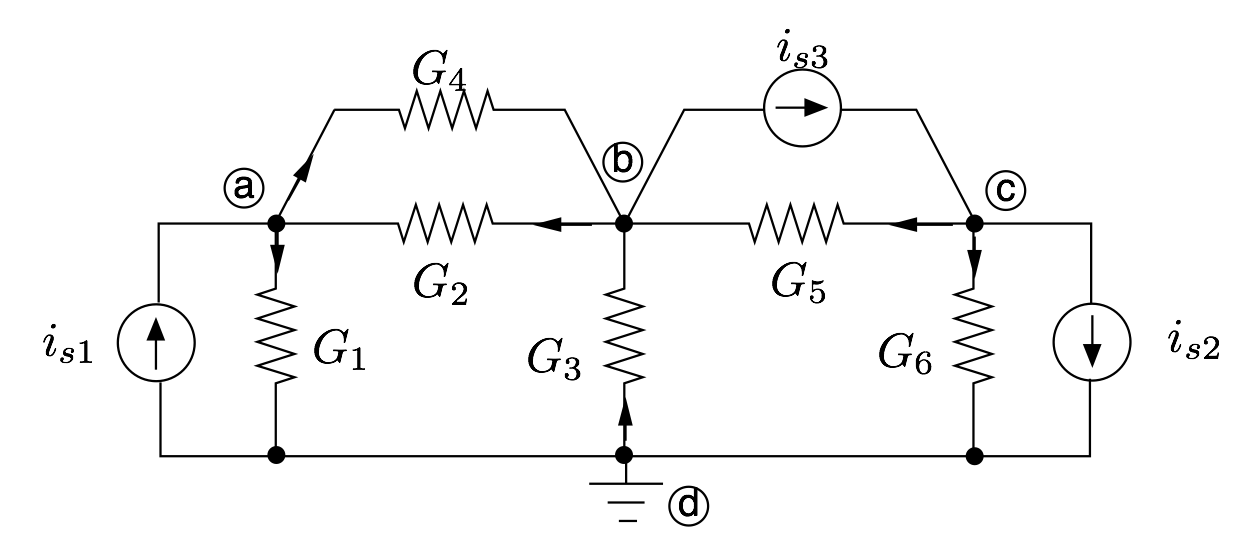
\includegraphics[width=0.7\linewidth]{figs/methodes-generales/exemple_iSN}
\end{center}
on a 
\[
i_1 =  G_1 u_{1}, \quad 
i_2 =  G_2 u_{2}, \quad 
\ldots , \quad 
i_6 =  G_6 u_{6}
\quad \Longleftrightarrow \quad {\bf i}_B = {\bf G}_B {\bf u}_B
\]
et donc 
\[\begin{array}{rcl}
G_1 u_1-G_2 u_2+G_4 u_4 & = & i_{s1}\\
G_2 u_2-G_3 u_3-G_4 u_4-G_5 u_5 & = & -i_{s3}\\
G_5 u_5+G_6 u_6 & = & i_{s3}-i_{s2}
\end{array}
\quad \Longleftrightarrow \quad {\bf A}\,{\bf G}_B{\bf u}_B = {\bf i}_{sN}
\]
\end{testexample}

\paragraph{Matrice de conductance aux noeuds.} %
Comme illustré aux étapes (\ref{eq:MN_5}) et (\ref{eq:MN_6}) de la dérivation de la méthode des noeuds, on peut remplacer les tensions de branches ${\bf u}_B$ par les potentiels de noeuds ${\bf v}_N$ :
\begin{testexample}[Matrice de conductance aux noeuds.] Pour le même exemple que celui qui a servi à illustrer $\mathbf{G}_B$, on a 

$$u_1 =  v_a, \quad 
u_2 =  v_b-v_a, \quad 
\ldots, \quad 
u_6 =  v_c$$
ou encore 
$$ {\bf u}_B = {\bf A}^T {\bf v}_N, $$
et donc 
\begin{gather*}
\begin{array}{rcl}
	(G_1+G_2+G_4) v_a-(G_2+G_4)v_b& = & i_{s1}\\
	-(G_2+G_4)v_a+(G_2+G_3+G_4+G_5)v_b-G_5 v_c & = & -i_{s3}\\
	-G_5 v_b+ (G_5+G_6) v_c & = & i_{s3}-i_{s2}
\end{array} 
\end{gather*}
ce qui se traduit sous forme matricielle par
\begin{center}
	$\underbrace{{\bf A}\,{\bf G}_B {\bf A}^T}_{{\bf G}_N}{\bf v}_N = {\bf i}_{sN}$
\end{center}
\end{testexample}

Ceci illustre une première manière de construire la matrice de conductance aux noeuds : 
\begin{enumerate}
\item construire $\mathbf{A}$,
\item construire $\mathbf{G}_B$,
\item calculer $\mathbf{G}_N = {\bf A}\,{\bf G}_B {\bf A}^T$
\end{enumerate}
Il existe des méthodes parfois plus directes pour construire $\mathbf{G}_N$.

\subsection{Détermination de $\mathbf{G}_N$ par inspection}
Appliquer $${\bf G}_N= {\bf A} {\bf G}_B {\bf A}^T$$ revient, lorsque $\mathbf{G}_B$ est diagonale\footnote{Ce qui n'est pas le cas avec des sources commandées.}, à appliquer la règle d'inspection de la Table~\ref{tab:inspectionG} : 
\begin{table}
\caption{Règle d'inspection pour déterminer les éléments de $\mathbf{G}_N$.}\label{tab:inspectionG}
\begin{boxedminipage}{\textwidth}
\begin{itemize}
	\item $G_{ii}$ est la somme des conductances des branches incidentes au
	noeud~$i$
	\item $G_{ik}$ est l'opposé de la somme des
	conductances des branches liant les noeuds $i$ et $k$
\end{itemize}
\end{boxedminipage}
\end{table}

\begin{testexample}[Détermination de $\mathbf{G}_N$ par inspection.]
Pour l'exemple précédent, on a directement 
\[
{\bf G}_N =
\left[ \begin{array}{ccc}
G_1+G_2+G_4 & -(G_2+G_4) & 0 \\
-(G_2+G_4) & G_2+G_3+G_4+G_5 & -G_5\\
0 & -G_5 & G_5+G_6
\end{array} \right]. \]
\end{testexample}

\subsection{Réseau équivalent}
Lorsque le circuit est mis en équation grâce à la méthode des noeuds, il peut être remplacé par un circuit équivalent constitué du
circuit passifié vu de $n-1$ accès auxquels agissent des sources
indépendantes de courant équivalentes regroupant les sources
indépendantes du circuit original (Figure~\ref{fig:reseau_equivalent_MN}).
\begin{figure}[htb]
	\centering
	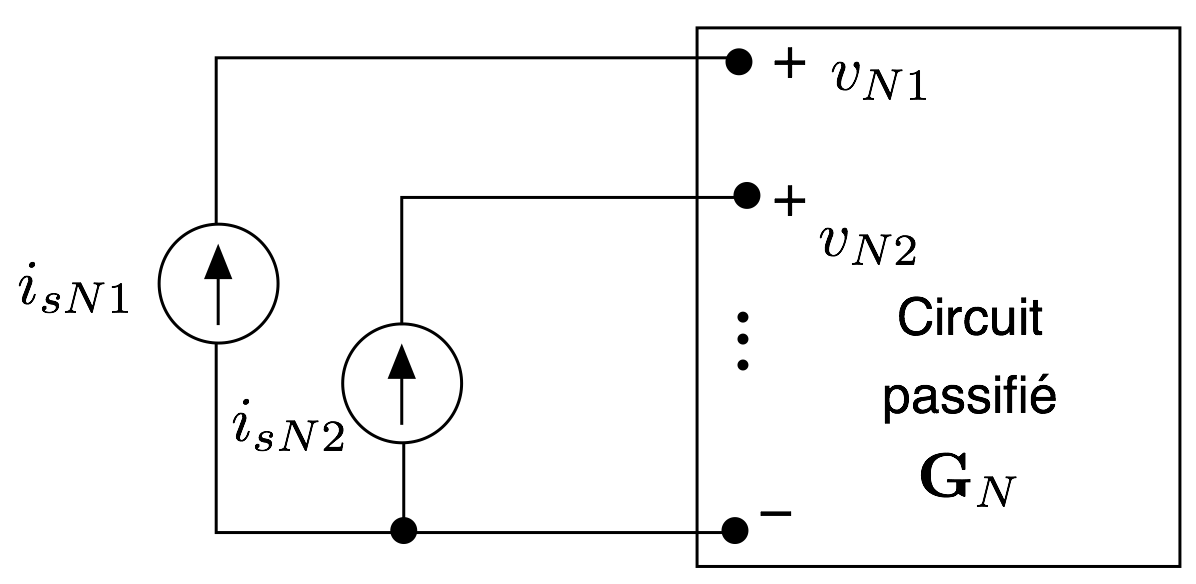
\includegraphics[width=0.6\linewidth]{figs/methodes-generales/reseau_equivalent_MN}
	\caption{Réseau équivalent.}
	\label{fig:reseau_equivalent_MN}
\end{figure}
Il s'agit d'un réseau passifié avec un accès entre chaque noeud et le noeud de
référence, et une source indépendante de courant agissant à chaque accès. correspondant aux composantes de ${\bf i}_{sN}$.
\begin{testexample}[Réseau équivalent.]
	\centering
	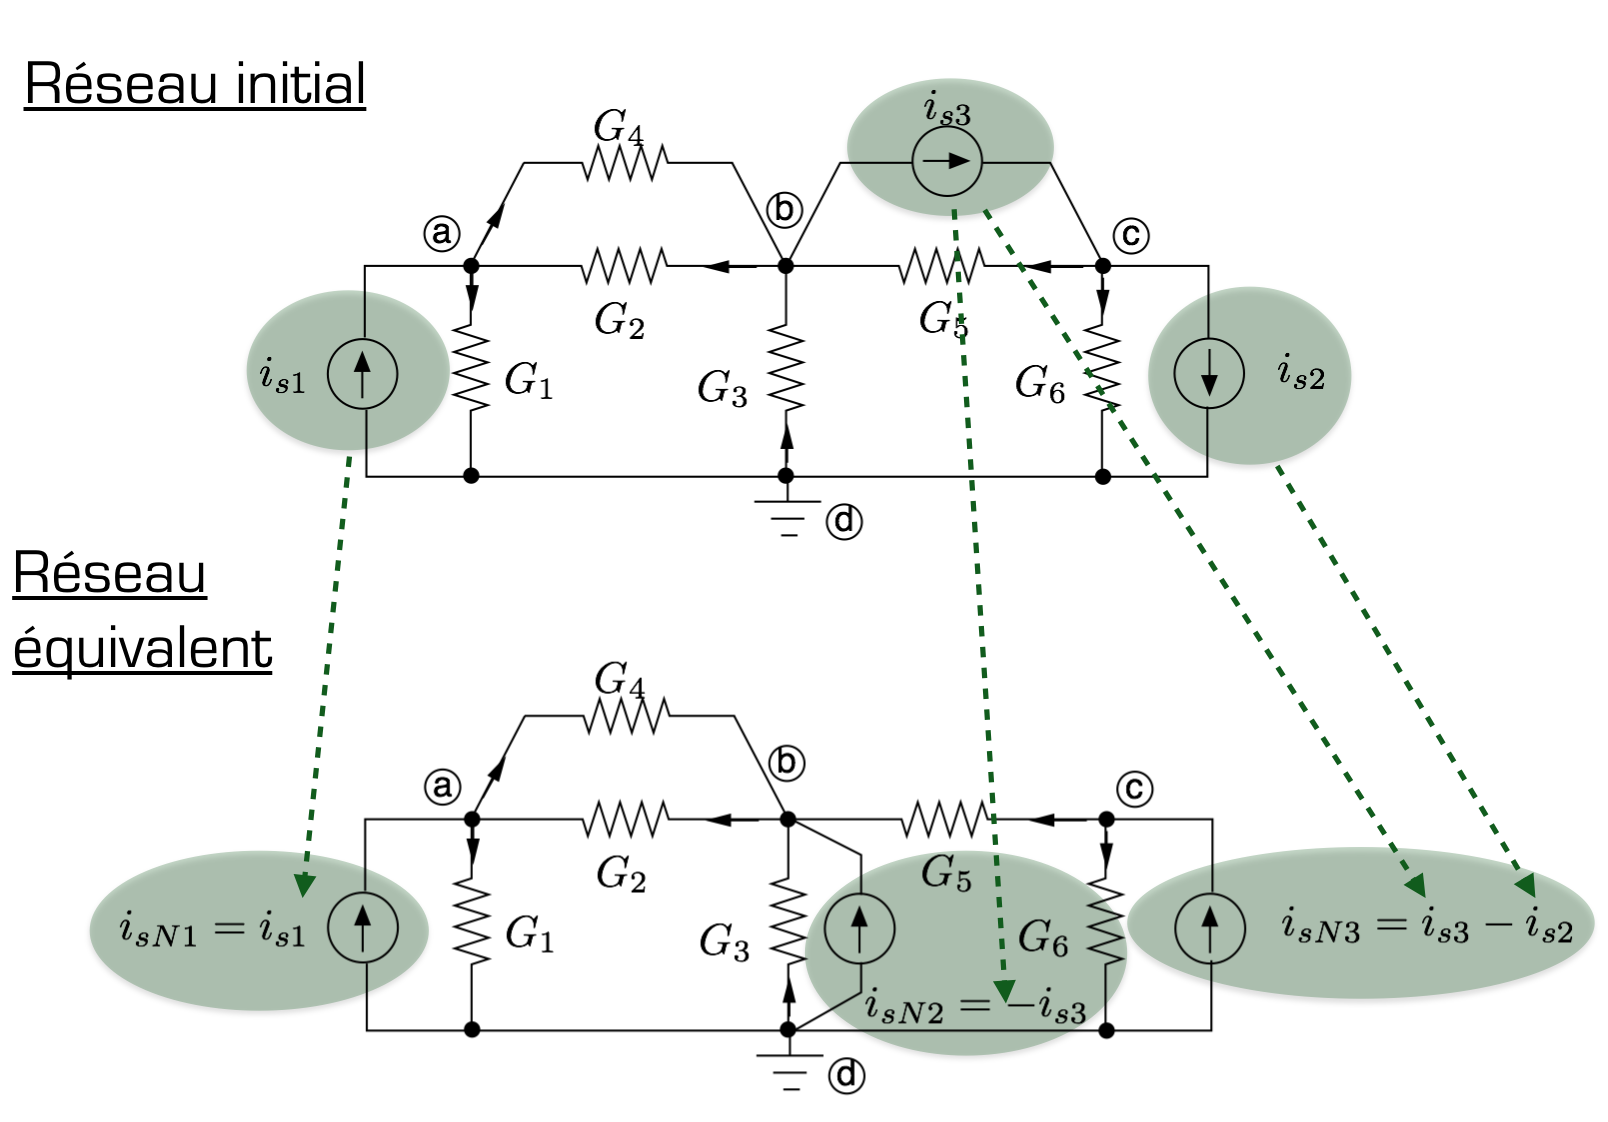
\includegraphics[width=0.9\linewidth]{figs/methodes-generales/ex_reseau_equivalent_MN}
\end{testexample}

\subsection{Détermination de $\mathbf{G}_N$ par expérimentation}
La dernière méthode pour déterminer $\mathbf{G}_N$ consiste à exploiter la représentation du circuit par un réseau équivalent. En effet, ${\bf G}_N$ caractérise le circuit passifié. Les relations $i-u$ aux $n-1$ accès s'écrivent : 
\begin{eqnarray*}
	i_{1} & = & G_{11}v_{1} + G_{12}v_{2}+ \ldots \\
	i_{2} & = & G_{21}v_{1} + G_{22}v_{2}+ \ldots 
\end{eqnarray*}
où ${\bf i}$ est le vecteur des courants injectés aux
accès, ${\bf v}$ est le vecteur des tensions aux accès.
\begin{marginfigure}[-2cm]
	\centering
	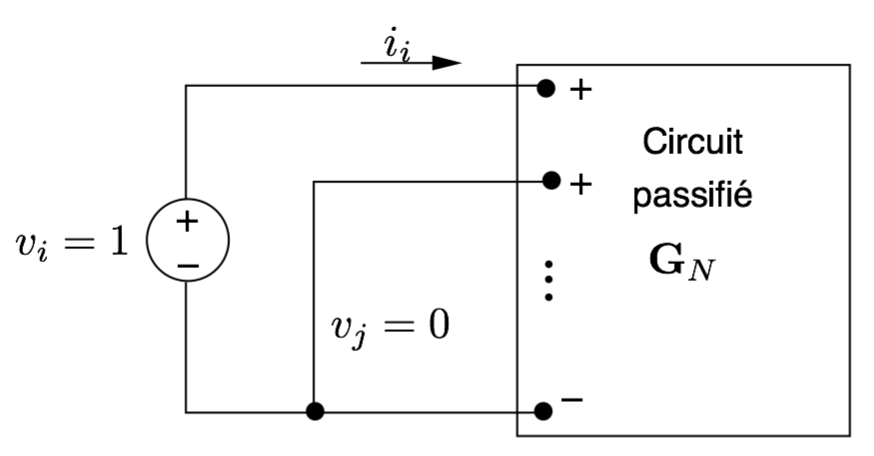
\includegraphics[width=\linewidth]{figs/methodes-generales/experimentation_ii} 
	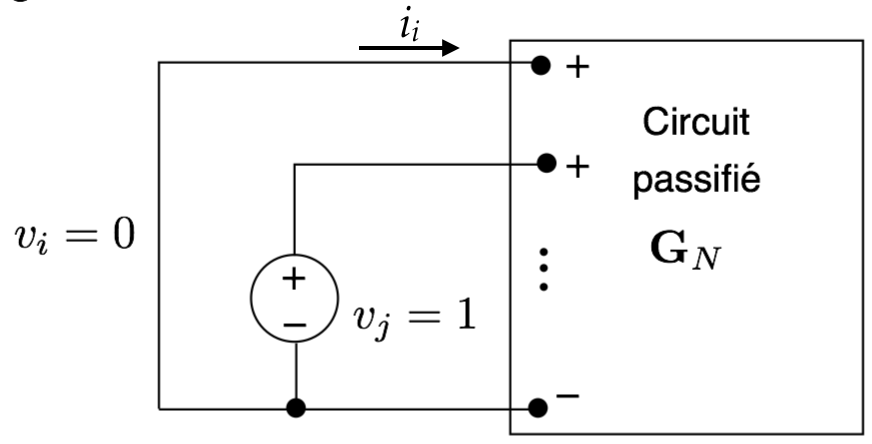
\includegraphics[width=0.95\linewidth]{figs/methodes-generales/experimentation_ij}
	\caption{Illustration de la méthode d'expérimenation pour les éléments diagonaux (haut) et hors diagonale (bas).}
	\label{fig:experimentation}
\end{marginfigure}

Les éléments de ${\bf G}_N$ sont alors déterminés par des essais
successifs, cf. Figure~\ref{fig:experimentation} et Table~\ref{tab:experimentation_G}. Cette méthode se révèle incontournable quand le circuit comporte des couplages entre branches ou quand, tout simplement, on n'a pas accès aux paramètres du circuit et on l'identifie par des mesures "physiques".
\begin{table}[htb]
	\caption{Règle d'expérimentation pour déterminer les éléments de $\mathbf{G}_N$.}\label{tab:experimentation_G}
	\begin{boxedminipage}{\textwidth}
\[G_{ij}= i_{i}|_{v_{j}=1, v_{k}=0,k\neq j}\]
\begin{itemize}
	\item Imposer une tension de $1 V$ à l'accès $j$
	\item Court-circuiter les autres accès
	\item Déterminer dans ces conditions le courant à l'accès $i$
\end{itemize}
\end{boxedminipage}
\end{table}

\begin{testexample}
Soit le circuit de la figure suivante, comportant une source VCT :
\begin{center}
	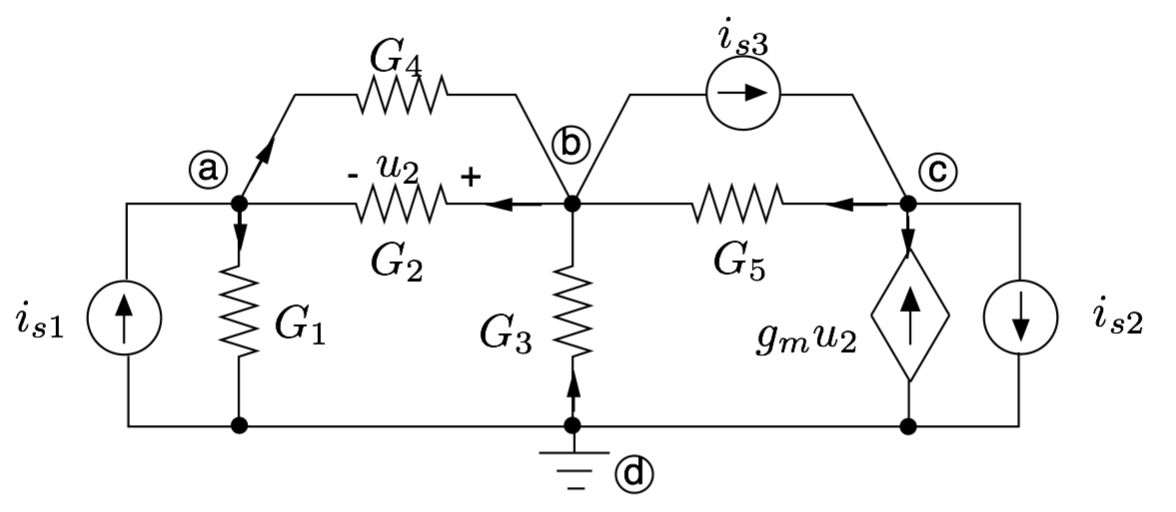
\includegraphics[width=0.7\linewidth]{figs/methodes-generales/ex_exp_0}
\end{center}
Calculons quelques éléments de ${\bf G}_N$. Commençons par 
\[G_{31}=i_{3}|_{v_{1}=1,v_{2}=v_{3}=0}\]
ce qui se traduit par l'expérience suivante : 
\begin{center}
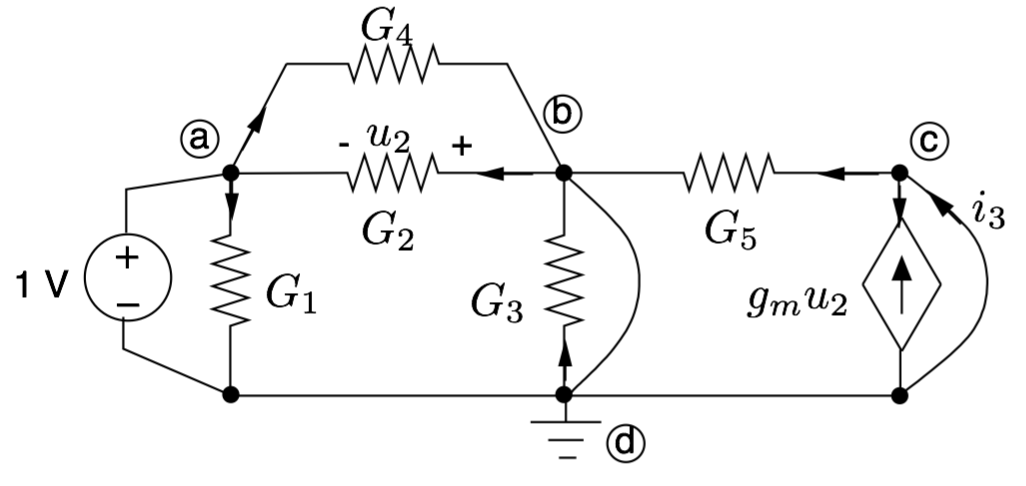
\includegraphics[width=0.7\linewidth]{figs/methodes-generales/ex_exp_1}
\end{center}
On a successivement 
\begin{align*}
u_5&=0 \\
i_5&=0 \\
u_2&=-1 \\
i_6&=-g_mu_2=g_m \\
G_{31} &= i_{3}= i_5+i_6=g_m
\end{align*}
De même pour \[G_{32}=i_{3}|_{v_{2}=1,v_{1}=v_{3}=0}\]
\begin{center}
	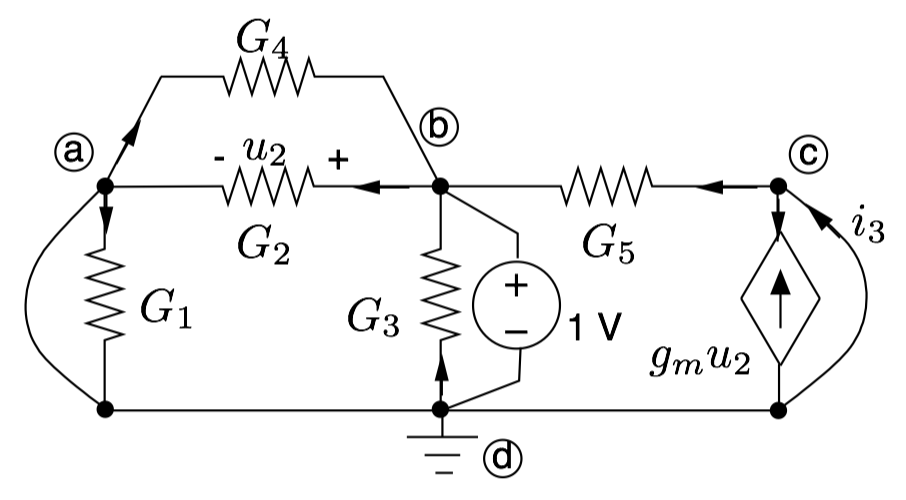
\includegraphics[width=0.7\linewidth]{figs/methodes-generales/ex_exp_2}
\end{center}
on a 
\begin{align*}
u_5&=-1 \\
i_5&=-G_5 \\
u_2&=1 \\
i_6&=-g_mu_2=-g_m\\
G_{32} & =  i_{3}= i_5+i_6 =  -(G_5+g_m)
\end{align*}
Finalement, pour \[G_{33}=i_{3}|_{v_{3}=1,v_{1}=v_{2}=0}\]
\begin{center}
	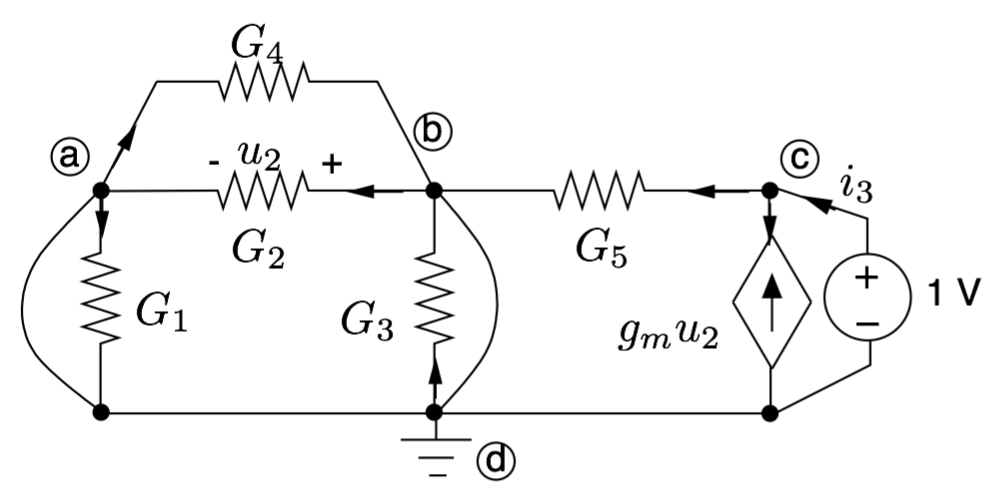
\includegraphics[width=0.7\linewidth]{figs/methodes-generales/ex_exp_3}
\end{center}
on a
\begin{align*}
u_5&=1 \\
i_5&=G_5 \\
u_2&=0 \\
i_6&=0 \\
G_{33} &= i_{3}= i_5+i_6=G_5.
\end{align*}
\end{testexample}


\subsection{Gestion des sources dépendantes de type VCT}
L'exemple de la section précédente nous a montré comment gérer une source de type VCT. On peut également les traiter avec la méthode de base, lors de la construction de la matrice $\mathbf{G}_B$, la matrice ${\bf A}$ étant indépendante de la nature des éléments qui constituent les branches. 

\begin{testexample}
Soit le circuit de la figure suivante, comportant une source VCT :
\begin{center}
	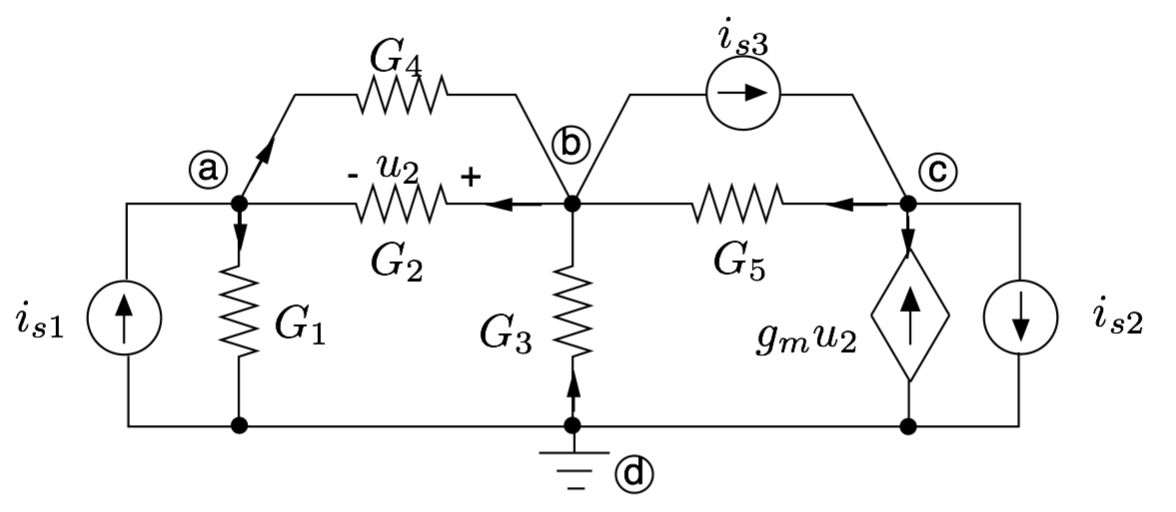
\includegraphics[width=0.7\linewidth]{figs/methodes-generales/ex_exp_0}
\end{center}
\[{\bf G}_B=
\left[
\begin{array}{cccccc}
G_1 & 0 & 0 & 0 & 0 & 0\\
0 & G_2 & 0 & 0 & 0 & 0 \\
0 & 0 & G_3 & 0 & 0 & 0\\
0 & 0 & 0 & G_4 & 0 & 0\\
0 & 0 & 0 & 0 & G_5 & 0\\
0 & -g_m& 0 & 0 & 0 & 0
\end{array}\right]\]

Dès lors, 
\[{\bf G}_N={\bf A}{\bf G}_B{\bf A}^T= 
\left[
\begin{array}{ccc}
G_1+G_2+G_4 & -(G_2+G_4) & 0 \\
-(G_2+G_4) & G_2+G_3+G_4+G_5 & -G_5 \\
g_m & -(G_5+g_m) & G_5
\end{array}\right]\]

${\bf G}_B$ et  ${\bf G}_N$ ne sont plus des matrices symétriques.
\end{testexample}

Par contre,  ${\bf G}_N$ ne peut plus être déterminée par inspection, ou en tous les cas pas totalement\footnote{Dans l'exemple précédent, on peut se rendre compte que la source VCT agit sur le courant injecté au noeud $c$ en fonction du potentiel des noeuds $a$ et $b$, d'où le fait que seuls les éléments de la ligne $3$ ($c$) et des colonnes $1$ ($a$) et $2$ ($b$) soient impactés.}.

\subsection{Gestion des sources indépendantes de tension}

Pour gérer les sources indépendantes de tension, on peut transformer le circuit comme suit : 
\begin{itemize}
	\item si une source est en série avec une résistance,  transformer la source de tension en une source de courant équivalente
	\item si une source est seule dans une branche, transformer le circuit comme indiqué à la Figure~\ref{fig:transformation_SIV}.
\end{itemize}
\begin{figure}[htb]
\centering
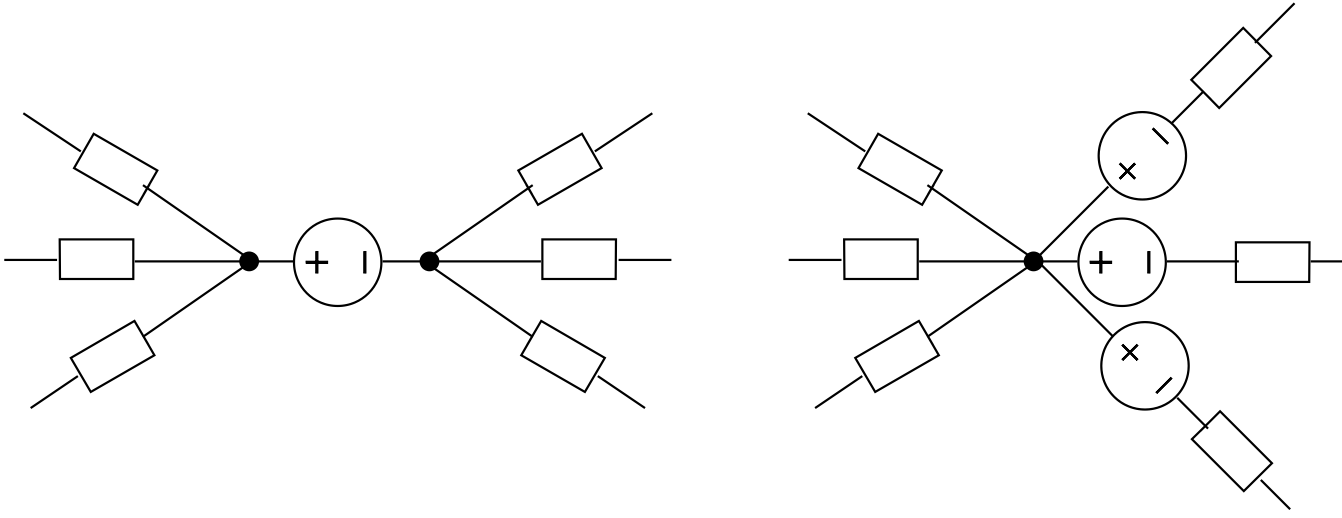
\includegraphics[width=0.95\linewidth]{figs/methodes-generales/transformation_SIV}
\caption{Gestion des sources indépendantes de tension dans la méthode des noeuds.}
\label{fig:transformation_SIV}
\end{figure}

On vérifie que dans le reste du circuit, les lois de Kirchhoff sont inchangées. La branche dans laquelle se trouve la f.e.m. ne doit pas être couplée avec le reste du circuit (par une source commandée par exemple).

\subsection{Généralisation du Théorème de Norton à plusieurs accès}
Considérons le schéma équivalent du circuit déduit de la méthode des noeuds (Figure~\ref{fig:nortonMM}), avec $N=n-1$ accès ; un accès entre chaque noeud et le noeud de référence, aux bornes de chaque source équivalente de courant.
Les relations $i-u$ pour les $N$ accès sont
\[{\bf i}=-{\bf i}_{sN}+{\bf G}_N{\bf v}_N\]
ou encore
\[{\bf i}=-{\bf i}_{sN}+{\bf G}_N{\bf u}\]
On en déduit le schéma équivalent de Norton à $N$ accès par simple identification :
\[ {\bf i}_{No} = {\bf i}_{sN}\,\, , \quad \quad {\bf G}_{No}={\bf G}_{N}\]
\begin{figure}[htb]
\centering
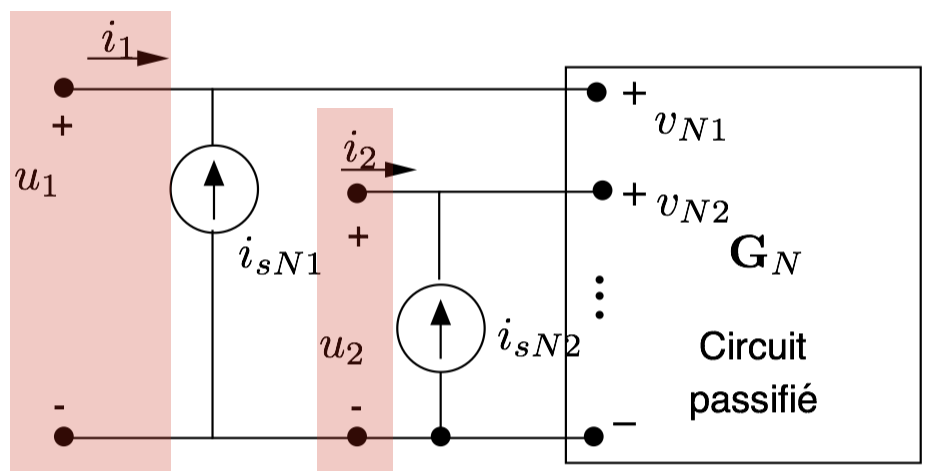
\includegraphics[width=0.7\linewidth]{figs/methodes-generales/norton}
\caption{Généralisation du Théorème de Norton à plusieurs accès.}
\label{fig:nortonMM}
\end{figure}

\subsection{Réduction du nombre d'accès}
On cherche à obtenir un schéma équivalent de Norton à $a$ accès (intéressants), avec $a<N$.
Les $N-a$ accès inintéressants sont laissés ouverts (ce qui ne dénature pas la topologie du circuit) : 
\[i_{a+1},\ldots,i_N=0\]
\begin{figure}[htb]
\centering
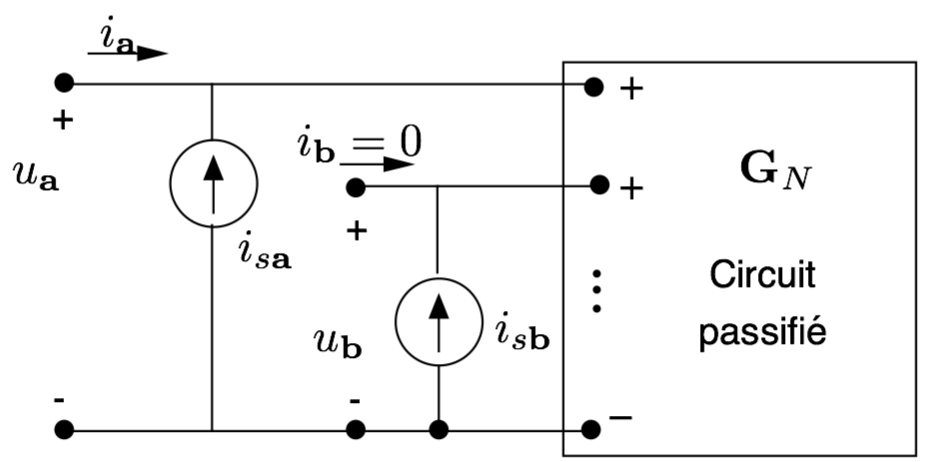
\includegraphics[width=0.7\linewidth]{figs/methodes-generales/reduction}
\caption{Illustration de la réduction du nombre d'accès.}
\label{fig:reduction}
\end{figure}
Utilisons les indices $\mathbf{a}$ et $\mathbf{b}$ pour partitionner les vecteurs en parties intéressantes et non-intéressantes. Les relations $i-u$ de la méthode des noeuds deviennent : 
{
\[\left[
\begin{array}{c}
{\bf i}_{\bf a}\\
{\bf i}_{\bf b}
\end{array}\right]=
- \left[
\begin{array}{c}
{\bf i}_{s{\bf a}}\\
{\bf i}_{s{\bf b}}
\end{array}\right] + 
\left[
\begin{array}{cc}
{\bf G}_{\bf a,a}& {\bf G}_{\bf a,b}\\
{\bf G}_{\bf b,a}& {\bf G}_{\bf b,b}
\end{array}\right]
\left[
\begin{array}{c}
{\bf u}_{\bf a}\\
{\bf u}_{\bf b}
\end{array}\right]\]
Par hypothèse, 
\[
{\bf i}_{\bf b}=0 =-{\bf i}_{s{\bf b}}+{\bf G}_{\bf b,a}{\bf u}_{\bf a}+{\bf
	G}_{\bf b,b}{\bf u}_{\bf b}\]
Donc 
\[{\bf u}_{\bf b}={\bf G}_{\bf b,b}^{-1}({\bf i}_{s{\bf b}}-{\bf G}_{\bf	b,a}{\bf u}_{\bf a})\]
et 
\[{\bf i}_{\bf a}=(-{\bf i}_{s{\bf a}}+{\bf G}_{\bf a,b}{\bf G}_{\bf b,b}^{-1}{\bf
	i}_{s{\bf b}})
+({\bf G}_{\bf a,a}-{\bf G}_{\bf a,b}{\bf G}_{\bf b,b}^{-1}{\bf
	G}_{\bf b,a}){\bf
	u}_{\bf a}\]
Finalement, comme on souhaite établir un modèle du type 
\[ {\bf i}_{\bf a}=-{\bf i}_{No}+{\bf G}_{No}{\bf u}_{\bf a}\]}
on a 

\begin{itemize}
\item le vecteur des sources équivalentes de Norton :
\[{\bf i}_{No}={\bf i}_{s{\bf a}}-{\bf G}_{\bf a,b}{\bf G}_{\bf b,b}^{-1}{\bf
	i}_{s{\bf b}}\]
c'est le vecteur des courants parcourant les  accès court-circuités (${\bf u}_{\bf a}={\bf 0}$)
\item la matrice de conductances  de Norton, soit la 
matrice de conductances ``réduite'' aux accès :
\[{\bf G}_{No}={\bf G}_{\bf a,a}-{\bf G}_{\bf a,b}{\bf G}_{\bf b,b}^{-1}{\bf
	G}_{\bf b,a}\]
qui peut être déterminée par expérimentation, mais jamais par inspection.
\end{itemize}

\begin{testexample}[Conversion étoile-triangle.]
Un circuit en étoile à trois branches peut être remplacé par un
circuit équivalent en triangle et inversement :
\begin{center}
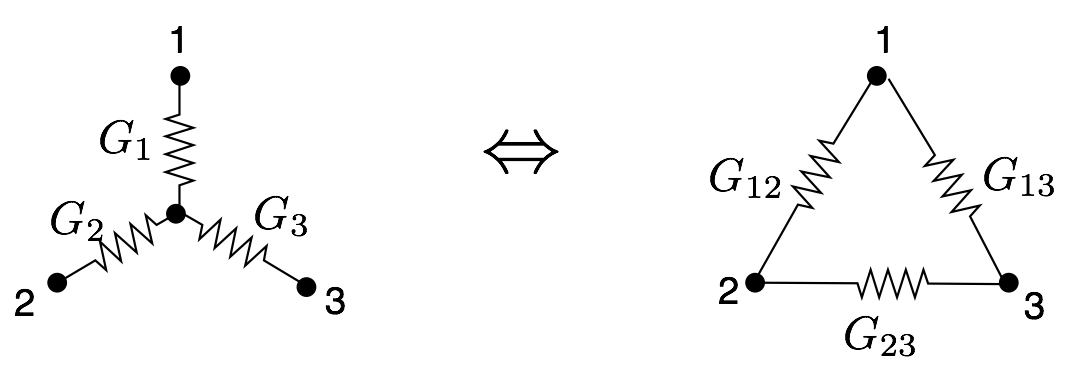
\includegraphics[width=0.9\linewidth]{figs/methodes-generales/e2t_3}
\end{center}
La condition d'équivalence est que les deux circuits aient la même matrice de conductances vue de deux accès (par exemple, $1-3$ et $2-3$)

La matrice de conductances aux accès du triangle ${\bf G}_T$ est la matrice de conductances au noeuds du circuit avec $3$ comme
noeud de référence :
\begin{center}
\begin{minipage}[c]{0.33 \textwidth}
	\begin{center}
	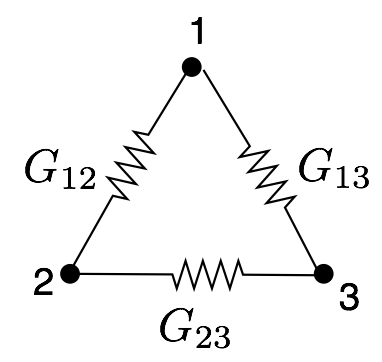
\includegraphics[width=0.9\linewidth]{figs/methodes-generales/e2t_2}
	\end{center}
\end{minipage}
\begin{minipage}[c]{0.66 \textwidth}
	\[{\bf G}_T=
	\left[
	\begin{array}{cc}
	G_{12}+G_{13} & -G_{12}\\
	-G_{12} & G_{12}+G_{23}
	\end{array} \right]\]
\end{minipage}
\end{center}

Construisons maintenant la matrice de conductances aux noeuds du triangle ${\bf G}_{NE}$ avec $3$ comme noeud de référence.
\begin{center}
	\begin{minipage}[c]{0.33 \textwidth}
		\begin{center}
			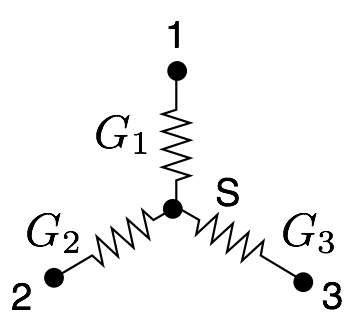
\includegraphics[width=0.9\linewidth]{figs/methodes-generales/e2t_1}
		\end{center}
	\end{minipage}
	\begin{minipage}[c]{0.66 \textwidth}
	\[{\bf G}_{NE}=
	\begin{array}{c}
	1 \\2 \\S
	\end{array}
	\left[
	\begin{array}{cc|c}
	G_1 & 0 & -G_1\\
	0 & G_2 & -G_2\\ \hline
	-G_1 & -G_2 & G_1+G_2+G_3
	\end{array} \right]\]
	\end{minipage}
\end{center}
	
Éliminons l'accès $S-3$ en réduisant ${\bf G}_{NE}$ aux 2 accès
``intéressants'' : 
\begin{eqnarray*}
	{\bf G}_E &=&
	\left[
	\begin{array}{cc}
		G_1 & 0\\ 0 & G_2
	\end{array} \right] - \left[
	\begin{array}{c}
		-G_1 \\-G_2
	\end{array}\right] \frac{1}{G_1+G_2+G_3} \left[
	\begin{array}{cc}
		-G_1 & -G_2
	\end{array}\right] \\[6mm] & = & \left[ 
	\begin{array}{cc}\displaystyle 
		\frac{G_1G_2+G_1G_3}{G_1+G_2+G_3} & \displaystyle 
		-\frac{G_1G_2}{G_1+G_2+G_3}\\\displaystyle 
		-\frac{G_1G_2}{G_1+G_2+G_3} & \displaystyle \frac{G_1G_2+G_2G_3}{G_1+G_2+G_3} 
	\end{array}\right]
\end{eqnarray*}
Par identification, on a  pour la transformation étoile $\rightarrow$ triangle :
\[\begin{array}{c}
G_{12}=\frac{G_1G_2}{G_1+G_2+G_3}\\[4mm]
G_{13}=\frac{G_1G_3}{G_1+G_2+G_3}\\[4mm]
G_{23}=\frac{G_2G_3}{G_1+G_2+G_3}
\end{array}\]
ou en utilisant les résistances des branches : 
\[\begin{array}{c}
R_{12}=\frac{R_1R_2+R_2R_3+R_1R_3}{R_3}\\[4mm]
R_{13}=\frac{R_1R_2+R_2R_3+R_1R_3}{R_2}\\[4mm]
R_{23}=\frac{R_1R_2+R_2R_3+R_1R_3}{R_1}
\end{array} \]
On peut de la même manière établir les conditions pour la transformation inverse.
\end{testexample}

\section{La méthode des mailles}
\label{sec:MM}

La méthode des mailles exploite la SLK et les variables principales sont les courants de maille. L'exposé de cette méthode suit la même structure que celui de la méthode des noeuds.


\subsection{Vue générale de la méthode}
Pour déterminer l'état électrique d'un système, la méthode des mailles consiste à résoudre le système linéaire suivant : 
$$\mathbf{R}_M \mathbf{i}_M = \mathbf{v}_{sM}.$$
où 
\begin{itemize}
	\item L'indice $M$ signifie "Maille".
	\item $\mathbf{v}_{sM}$ est le vecteur des sources indépendantes de tension agissant dans les mailles. Déterminé par inspection, il caractérise l'impact des sources indépendantes de tension.
	\item $\mathbf{i}_M$ est le vecteur des courants de maille. Il contient les $b-n-1$ variables du système, et les tensions de branches en découlent, via la loi d'Ohm.
	\item $\mathbf{R}_M$ est la matrice de résistances de mailles. Déterminée par inspection ou par expérimentation, elle caractérise le graphe du circuit passifié.
\end{itemize}

Algorithmiquement, la méthode se résume aux cinq étapes principales décrites dans la Table~\ref{tab:methode_mailles}.
\begin{table}[tb]
	\caption{Vue algorithmique de la méthode des mailles. \label{tab:methode_mailles}}
	\begin{boxedminipage}{\textwidth}
		\begin{enumerate}
			\item Choisir un arbre orienté dans le graphe du circuit de référence,
			\item déterminer la matrice $\mathbf{R}_M$,
			\item déterminer le vecteur $\mathbf{v}_{sM}$,
			\item résoudre le système $$\mathbf{R}_M \mathbf{i}_M = \mathbf{v}_{sM}$$ pour obtenir les courants de branches,
			\item déduire de $\mathbf{i}_M$ l'état du circuit.
		\end{enumerate}
	\end{boxedminipage}
\end{table}
Cette méthode est applicable si le circuit est linéaire et s'il ne comporte que des sources indépendantes de tension\footnote{ Nous verrons plus tard comment gérer les sources indépendantes de courant et les source commandées de courant (CVT).}.

\subsection{Dérivation de la méthode des noeuds}

Les trois relations suivantes, reposant sur la matrice des mailles et la matrice de résistance de branches, traduisent respectivement la SLK (\ref{eq:MM_1}), le lien entre courants de branche et courants de maille (\ref{eq:MM_2}), et la loi d'Ohm (\ref{eq:MN_3}) :
\begin{align}
\mathbf{B} \mathbf{u}_B &= \mathbf{v}_{sM} \label{eq:MM_1}\\
\mathbf{i}_B &= \mathbf{B}^T \mathbf{i}_{M} \label{eq:MM_2}\\
\mathbf{u}_B &= \mathbf{R}_B \mathbf{i}_{B} \label{eq:MM_3}
\end{align}
On établit ensuite le système résolu par la méthode des mailles sur base de ces trois relations par simples manipulations et en définissant la \textit{matrice de résistances de mailles} $\mathbf{R}_M.$
\begin{align}
(\ref{eq:MM_3}) \rightarrow (\ref{eq:MM_1}) \quad \mathbf{B} \mathbf{R}_B \mathbf{i}_{B} &= \mathbf{v}_{sM} \label{eq:MM_4}\\
(\ref{eq:MM_2}) \rightarrow (\ref{eq:MM_4}) \quad \mathbf{B} \mathbf{R}_B \mathbf{B}^T \mathbf{i}_{M} &= \mathbf{v}_{sM} \label{eq:MM_5}\\
\mathbf{R}_M &\triangleq \mathbf{B} \mathbf{R}_B \mathbf{B}^T \label{eq:MM_6}\\
(\ref{eq:MM_6}) \rightarrow (\ref{eq:MM_5}) \quad \mathbf{R}_M &\mathbf{i}_M = \mathbf{v}_{sM}
\end{align}

\subsection{Matrice des mailles}
C'est une formulation duale à celle de la matrice d'incidence réduite.
Nous considérons un graphe orienté à $n$ noeuds, $m$ mailles et $b$ branches et définissons des matrices décrivant les relations d'appartenance mailles-branches.

\paragraph{Matrice des mailles $\mathbf{B}_a$.} C'est une matrice d'ordre $m \times b$ où chaque élément $b_{ij}$ est défini comme suit:
\begin{enumerate}
	\item $b_{ij} = -1$ si la branche $j$ appartient à la maille $i$ et est orientée dans le même sens ;
	\item $b_{ij} = +1$ si la branche $j$ appartient à la maille $i$ et est orientée en sens opposé ;
	\item $b_{ij} = 0$ si la branche $j$ n'appartient pas à la maille $i$
\end{enumerate}

Contrairement à la matrice d'incidence complète dont le nombre de lignes est égal
à $n$ (nombre de noeuds du graphe), il n'existe pas d'expression analytique simple du nombre total de lignes de $\mathbf{B}_a$ (c'est-à-dire du nombre total de mailles) en fonction de $n$ et $b$.

\begin{testexample}[Matrice des mailles.]
	Soit le réseau ci-dessous et sa représentation sous forme de graphe orienté (à droite).
	\begin{center}
		\centering
		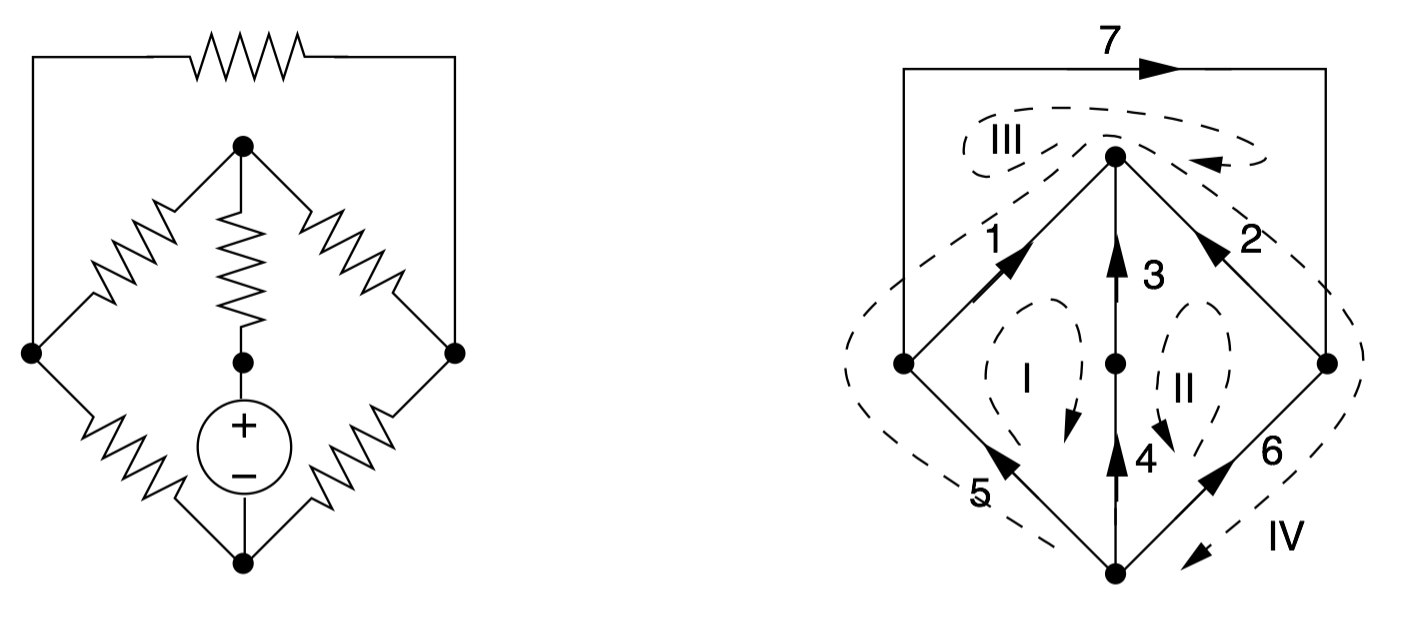
\includegraphics[width=0.9\linewidth]{figs/methodes-generales/m_mailles_1}
	\end{center}
	Il comporte $n=5$ noeuds, $b=7$ branches, et \underline{au moins} les $4$ mailles représentées. La SLK dans chacune de ces $4$ mailles s'écrit
	$$
	{\small
		\begin{array}{rcccccccccl}
		I & :&  - u_1&     & + u_3  & +  u_4  & -  u_5 &    &    & = &
		0\\ 
		II & : &     & -u_2&+ u_3& +  u_4  &        &-  u_6  &        &
		= & 0\\
		III & : &  + u_1  &-  u_2&     &     &     &  & -  u_7 & = &
		0 \\
		IV & : & -  u_1  &+   u_2  &   &  & -    u_5   &+  u_6  &   
		& = & 0
		\end{array}}
	$$
	On voit directement que la dernière ligne est la différence des deux premières.
\end{testexample}


\paragraph{Matrice des mailles fondamentales $\mathbf{B}$.}

Des mailles sont dites indépendantes lorsque les lignes de la matrice $\mathbf{B}_a$ qui leur sont associées sont elles-mêmes linéairement indépendantes. Il est évident que le nombre total de mailles comprises dans $\mathbf{B}_a$ est supérieur au nombre de mailles indépendantes.
Sur base des mailles fondamentales associées à un arbre ainsi que leur matrice correspondante, $\mathbf{B}$, en remarquant que ces mailles constituent un sous-ensemble des mailles incluses dans $\mathbf{B}_a$, on peut 
démontrer que ces mailles fondamentales sont les mailles indépendantes cherchées ;
les relations qu'elles fournissent permettent dès lors de reconstituer les relations branches-mailles de toutes les mailles du graphe.

Pour définir les mailles fondamentales associées à un arbre, on procède comme indiqué dans la Table~\ref{tab:mailles_fondamentales}.
\begin{table}[ht]
	\caption{Construction de la matrice des mailles fondamentales $\mathbf{B}$.\label{tab:mailles_fondamentales}}
\begin{boxedminipage}{\textwidth}
\begin{enumerate}
\item Identifier toutes les branches du graphe en réservant les premiers numéros (ou lettres) aux branches de l'arbre ;
\item former une maille fondamentale à partir d'un seul maillon et de branches de l'arbre ; son orientation coïncide avec celle du maillon ;
\item utiliser successivement tous les maillons, chacun une seule fois ;
\item numéroter les mailles fondamentales et disposer les lignes correspondantes en respectant le même ordre que celui utilisé pour la formation des colonnes relatives aux maillons correspondants.
\end{enumerate}
\end{boxedminipage}
\end{table}
La matrice $\mathbf{B}$ ainsi formée a $[b - (n - 1)]$ lignes et $b$ colonnes correspondant aux $b$ branches du graphe connexe.


\begin{testexample}[Matrice des mailles fondamentales.]
	Dans l'exemple précédent, choisissons l'arbre  formé des branches $1$, $2$, $3$ et $4$. 		
	\begin{center}
	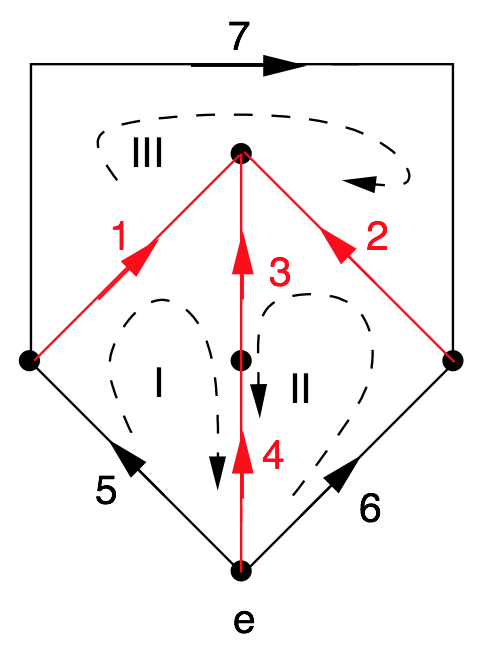
\includegraphics[width=0.4\linewidth]{figs/methodes-generales/m_mailles_2}
	\end{center}
	On a 
	\[ {\bf B} = 
	\left[\begin{array}{rrrrrrr}
	1 & 0 & -1 & -1 & 1 & 0 & 0\\
	0&1 & -1& -1 & 0  & 1 & 0\\
	-1 & 1 & 0 & 0 & 0  &0 &1
	\end{array}\right] \]
	Le rang de la matrice est $3=7-(5-1)$.
\end{testexample}
On peut maintenant écrire $${\bf B}\, {\bf u}_B =  {\bf 0},$$
avec $b-(n-1)$ relations linéairement indépendantes, où
${\bf u}_B$ est le vecteur des tensions de branches orientées selon le sens choisi pour construire ${\bf B}$.

\subsection{Vecteur des sources indépendantes de tension} Nous avons jusqu'à présent considéré le graphe passifié. Considérons maintenant l'impact des sources indépendantes de tension dans les mailles à travers le vecteur ${\bf v}_{sM}$. 

Un élément de ${\bf v}_{sM}$ est la  somme des tensions imposées dans chaque maille par les sources. Une source est prise avec le signe "$+$" si elle est orientée dans le sens de parcours de la maille, "$-$" sinon. 

Avec ces conventions, on a 
$${\bf B}\,{\bf u}_B = {\bf v}_{sM}$$

\begin{testexample}[Vecteur $\mathbf{v}_{sM}$.]
	Reprenons le circuit précédent et l'arbre illustré en rouge.
	\begin{center}
	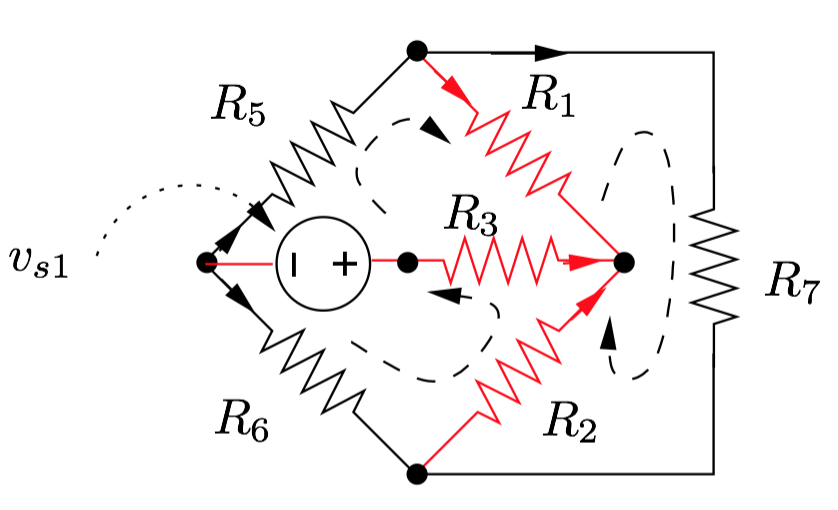
\includegraphics[width=0.5\linewidth]{figs/methodes-generales/m_mailles_3}
	\end{center}
	 La source de tension qui agit dans les mailles $I$ et $II$ est orientée en sens opposé à celui de ces mailles, donc  
	\[ {\bf v}_{sM} = 
	\left[
	\begin{array}{c}
	-v_{s1}\\
	-v_{s1}\\
	0
	\end{array} \right] \]
	En effet, par la SLK dans les trois mailles fondamentales, 
	\[\begin{array}{lrcl}
	I : & u_1-u_3+u_5 & = & -v_{s1}\\
	II : & u_2-u_3+u_6 & = & -v_{s1}\\
	III : & -u_1+u_2+u_7 & = & 0
	\end{array}
	\] est équivalent à  $${\bf B}\,{\bf u}_B = {\bf v}_{sM}.$$ 
\end{testexample}

\subsection{Courant de maille}
On appelle \textit{courant de maille} le courant "virtuel" circulant à travers une maille. C'est en fait le courant qui circule dans le maillon qui définit la maille.  La matrice des mailles fait le lien entre ces courants "virtuels" et les courants de branche : 
$$\mathbf{i}_B = \mathbf{B}^T \mathbf{i}_{M}.$$
Chaque courant est considéré selon le sens de parcours de la maille ou de la branche correspondante.
\begin{testexample}
	Soit le graphe suivant et l'arbre correspondant
	\begin{center}
	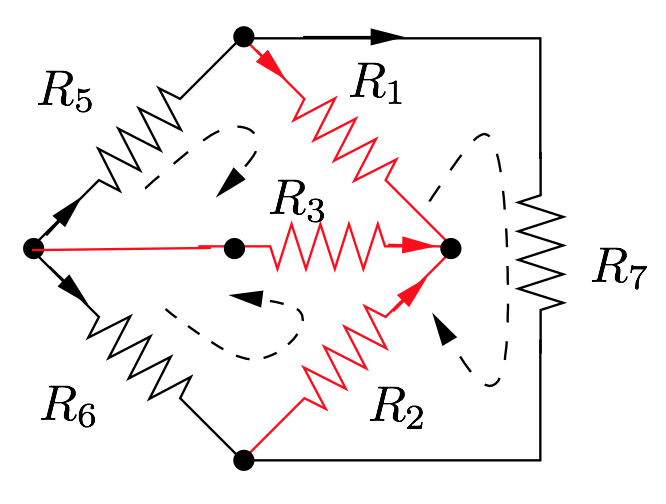
\includegraphics[width=0.4\linewidth]{figs/methodes-generales/m_mailles_4}
	\end{center}
	on a le vecteur ${\bf i}_M$ des courants dans les maillons : 
	$${\bf i}_M=\left[ i_5, i_6, i_7\right]^T$$
	et
	$$
		\left[\begin{array}{c}
		i_1 \\
		i_2 \\
		i_3 \\
		i_4 \\
		i_5 \\
		i_6 \\
		i_7 
		\end{array}\right] = 
		\left[\begin{array}{rrr}
		1 & 0 & -1 \\
		0 & 1 & 1 \\
		-1 & -1 & 0 \\
		-1 & -1 & 0 \\
		1 & 0 & 0  \\
		0 & 1 & 0 \\
		0 & 0 & 1 
		\end{array}\right]
		\left[\begin{array}{c}
		i_{I}\\
		i_{II}\\
		i_{III}
		\end{array}\right]$$	
\end{testexample}

\subsection{Matrice de résistance}
\paragraph{Matrice de résistance de branches.} %
L'application de la loi d'Ohm dans chaque branche permet de remplacer les tensions de branches ${\bf u}_B$ par les courants de branches ${\bf i}_B$. Si le circuit comporte uniquement des résistances linéaires, on définit la matrice de résistance de branches ${\bf R}_B$ de dimension $b \times b$ comme la matrice diagonale suivante
\[{\bf R}_B = \left[
\begin{array}{cccc}
R_1 & \\
& R_2 & {\bf 0} & \\
&  {\bf 0} & \ddots \\
& & & R_b
\end{array} \right]\]

\begin{testexample}
	Pour le circuit suivant
	\begin{center}
	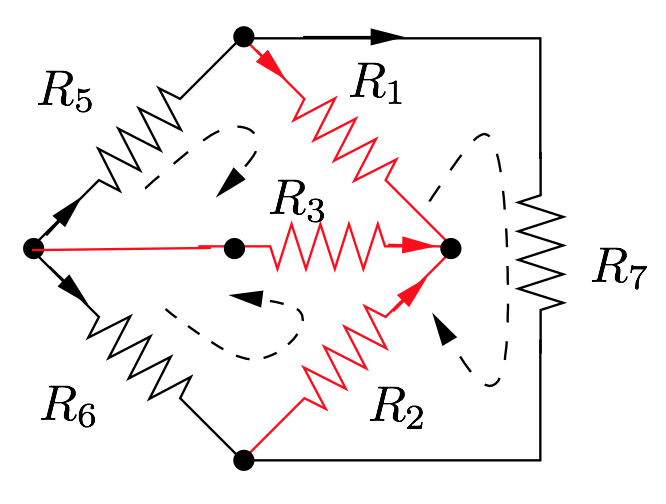
\includegraphics[width=0.4\linewidth]{figs/methodes-generales/m_mailles_4}
	\end{center}
	on a 
	{\small \[
	u_1 =  R_1 i_{1}, \quad 
	u_2 =  R_2 i_{2}, \quad 
	\ldots , \quad 
	u_7 =  R_7 i_{7}
	\quad \Longleftrightarrow \quad {\bf u}_B = {\bf R}_B {\bf i}_B
	\]
	\[\begin{array}{rcl}
	R_1 i_1-R_3 i_3+R_5 i_5 & = & -v_{s1}\\
	R_2 i_2-R_3 i_3+R_6 i_6 & = & -v_{s1}\\
	-R_1 i_1+R_2 i_2 + R_7 i_7 & = & 0
	\end{array}
	\quad \Longleftrightarrow \quad {\bf B}\,{\bf R}_B{\bf i}_B = {\bf v}_{sM}
	\]}
\end{testexample}

\paragraph{Matrice de résistance de mailles.} %
Comme illustré aux étapes (\ref{eq:MM_5}) et (\ref{eq:MM_6}) de la dérivation de la méthode des mailles, on peut remplacer les courants de branche ${\bf i}_B$ par les courants de maille ${\bf i}_M$.
\begin{testexample}[Matrice de résistance de mailles.] Pour le même exemple que celui qui a servi à illustrer $\mathbf{R}_B$, on a 
	$${\bf i}_B = {\bf B}^T {\bf i}_M$$ ou encore 
	$$i_1 =  i_{M1}-i_{M3} \quad 
	i_2 =  i_{M2}+i_{M3} \quad 
	\ldots \quad 
	i_7 =  i_{M3}$$
	et donc 
	\begin{gather*}
	\begin{array}{rcl}
	(R_1+R_3+R_5) i_{M1}+R_3 i_{M2}-R_1 i_{M3}& = & -v_{s1}\\
	R_3 i_{M1} + (R_2+R_3+R_6)i_{M2}+R_2 i_{M3} & = & -v_{s1}\\
	-R_1 i_{M1} + R_2 i_{M2} + (R_1+R_2+R_7) i_{M3} & = & 0
	\end{array}
	\end{gather*}
	ce qui se traduit sous forme matricielle par
	\begin{center}
		$\underbrace{{\bf B}\,{\bf R}_B {\bf B}^T}_{{\bf R}_M}{\bf i}_M = {\bf v}_{sM}$
	\end{center}
\end{testexample}

Ceci illustre une première manière de construire la matrice de résistance de maille : 
\begin{enumerate}
	\item construire $\mathbf{B}$,
	\item construire $\mathbf{R}_B$,
	\item calculer $\mathbf{R}_M = {\bf B}\,{\bf R}_B {\bf B}^T$
\end{enumerate}
Il existe des méthodes parfois plus directes pour construire $\mathbf{R}_M$.

\subsection{Détermination de $\mathbf{R}_M$ par inspection}
Appliquer $$\mathbf{R}_M = {\bf B}\,{\bf R}_B {\bf B}^T$$ revient, lorsque $\mathbf{R}_B$ est diagonale\footnote{Ce qui n'est pas le cas avec des sources commandées.}, à appliquer la règle d'inspection de la Table~\ref{tab:inspectionR}.	 
\begin{table}[ht]
	\caption{Règle d'inspection pour déterminer les éléments de $\mathbf{R}_M$.}\label{tab:inspectionR}
	\begin{boxedminipage}{\textwidth}
		\begin{itemize}
			\item $R_{ii}$ est la somme des résistances des branches de la maille ~$i$
			\item $R_{ik}$ est la somme des résistances des branches communes aux mailles $i$ et $k$, prises avec le signe $+$ si les sens de parcours des deux mailles coïncident, avec le signe $-$ dans le cas contraire.
		\end{itemize}
	\end{boxedminipage}
\end{table}

\begin{testexample}[Détermination de $\mathbf{R}_M$ par inspection.]
	Pour l'exemple précédent, on a directement 
	\[
	{\bf R}_M= 
	\left[ \begin{array}{ccc}
	R_1+R_3+R_5 & R_3 & -R_1 \\
	R_3 & R_2+R_3+R_6 & R_2 \\
	-R_1 & R_2 & R_1+R_2+R_7
	\end{array} \right] \]
\end{testexample}

\subsection{Réseau équivalent}
Lorsque le circuit est mis en équation grâce à la méthode des mailles, il peut être remplacé par un circuit équivalent constitué du
circuit passifié vu de $M=b-(n-1)$ accès auxquels agissent des sources
indépendantes de tension équivalentes regroupant les sources
indépendantes du circuit original (Figure~\ref{fig:reseau_equivalent_MM}).
\begin{figure}[htb]
	\centering
	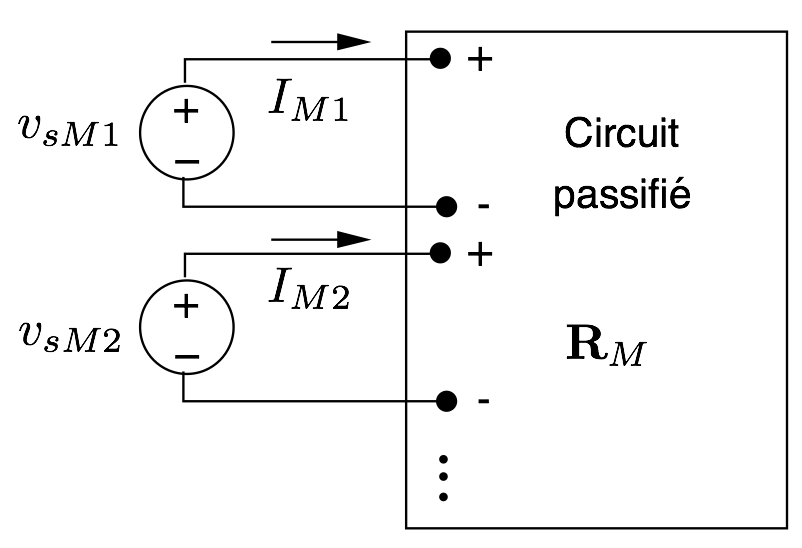
\includegraphics[width=0.5\linewidth]{figs/methodes-generales/MM_equivalent}
	\caption{Réseau équivalent.}
	\label{fig:reseau_equivalent_MM}
\end{figure}
Il s'agit d'un réseau passifié avec un accès à chaque maillon (on ouvre le maillon), et une source indépendante de tension agissant à chaque accès (on ferme les maillons) correspondant aux composantes de ${\bf v}_{sM}$.

\subsection{Détermination de $\mathbf{R}_M$ par expérimentation}
La dernière méthode pour déterminer $\mathbf{R}_M$ consiste à exploiter la représentation du circuit par un réseau équivalent. En effet, ${\bf R}_M$ caractérise le circuit passifié. Les relations $u-i$ aux $b-(n-1)$ accès s'écrivent : 
\begin{eqnarray*}
	u_{1} & = & R_{11}i_{1} + R_{12}i_{2}+ \ldots \\
	u_{2} & = & R_{21}i_{1} + R_{22}i_{2}+ \ldots 
\end{eqnarray*}
où ${\bf i}$ est le vecteur des courants injectés aux
accès, ${\bf u}$ est le vecteur des tensions aux accès.

\begin{marginfigure}[-1cm]
	\centering
	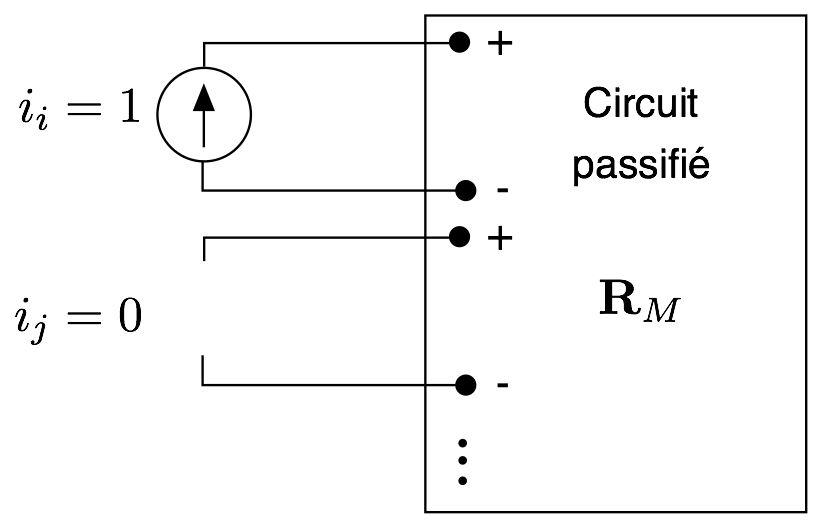
\includegraphics[width=\linewidth]{figs/methodes-generales/experimentation_MM_ii} 
	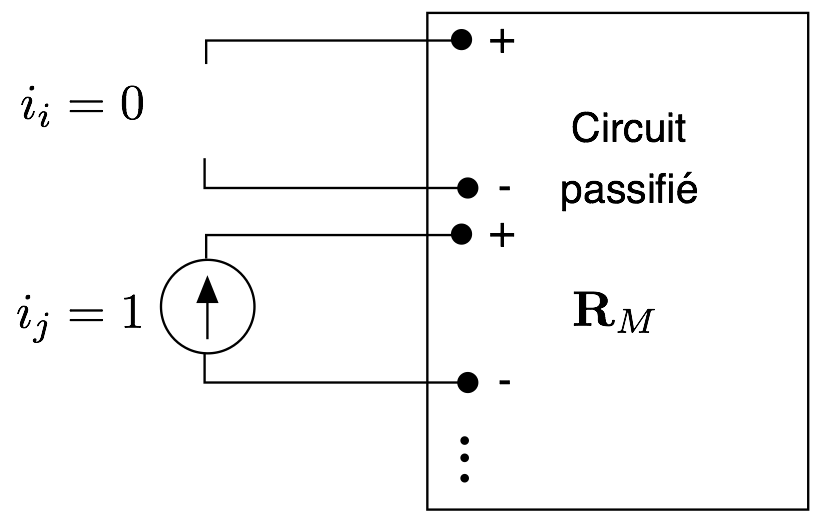
\includegraphics[width=\linewidth]{figs/methodes-generales/experimentation_MM_ij}
	\caption{Illustration de la méthode d'expérimenation pour les éléments diagonaux (haut) et hors diagonale (bas).}
	\label{fig:experimentation_MM}
\end{marginfigure}

Les éléments de ${\bf R}_M$ sont alors déterminés par des essais
successifs, cf. Figure~\ref{fig:experimentation_MM} et Table~\ref{tab:experimentation_MM}. Cette méthode se révèle incontournable quand le circuit comporte des couplages entre branches ou quand, tout simplement, on n'a pas accès aux paramètres du circuit et on l'identifie par des mesures "physiques".
\begin{table}[htb]
	\caption{Règle d'expérimentation pour déterminer les éléments de $\mathbf{R}_M$.}\label{tab:experimentation_MM}
	\begin{boxedminipage}{\textwidth}
		\[R_{ij}= u_{i}|_{i_{j}=1, i_{k}=0,k\neq j}\]
		\begin{enumerate}
			\item Imposer un courant  de $1 A$ à l'accès $j$
			\item Laisser les autres accès ouverts ($i=0$)
			\item Déterminer dans ces conditions la tension à l'accès $i$
		\end{enumerate}
	\end{boxedminipage}
\end{table}

\begin{testexample}
	Soit le circuit de la figure suivante, comportant une source CVT :
	\begin{center}
		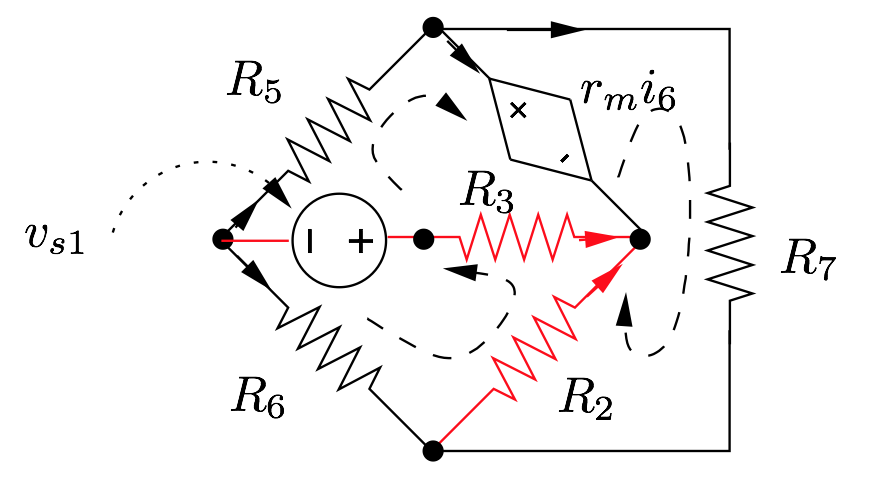
\includegraphics[width=0.5\linewidth]{figs/methodes-generales/ex_exp_MM_0}
	\end{center}
	Calculons quelques éléments de ${\bf R}_M$. Commençons par 
	$R_{11}=v_{I}|_{i_{I}=1,i_{II}=i_{III}=0}$
	ce qui se traduit par l'expérience suivante : 
	\begin{center}
		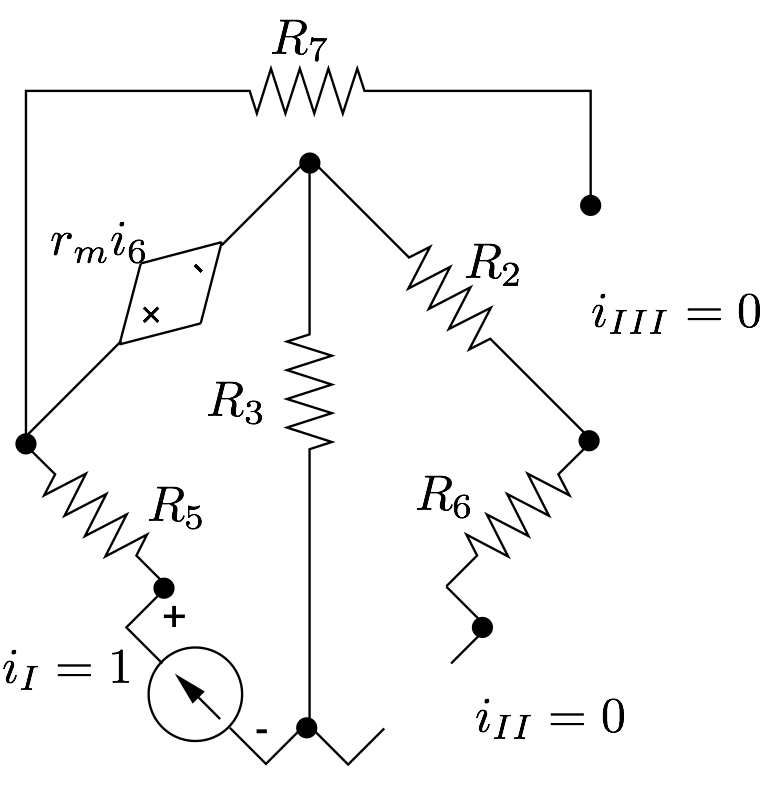
\includegraphics[width=0.4\linewidth]{figs/methodes-generales/ex_exp_MM_1}
	\end{center}
	On a $i_6=0$ et $R_{11} = v_{I}= R_5+R_3$.
	
	De même pour $R_{12}=v_{I}|_{i_{II}=1,i_{I}=i_{III}=0}$
	\begin{center}
		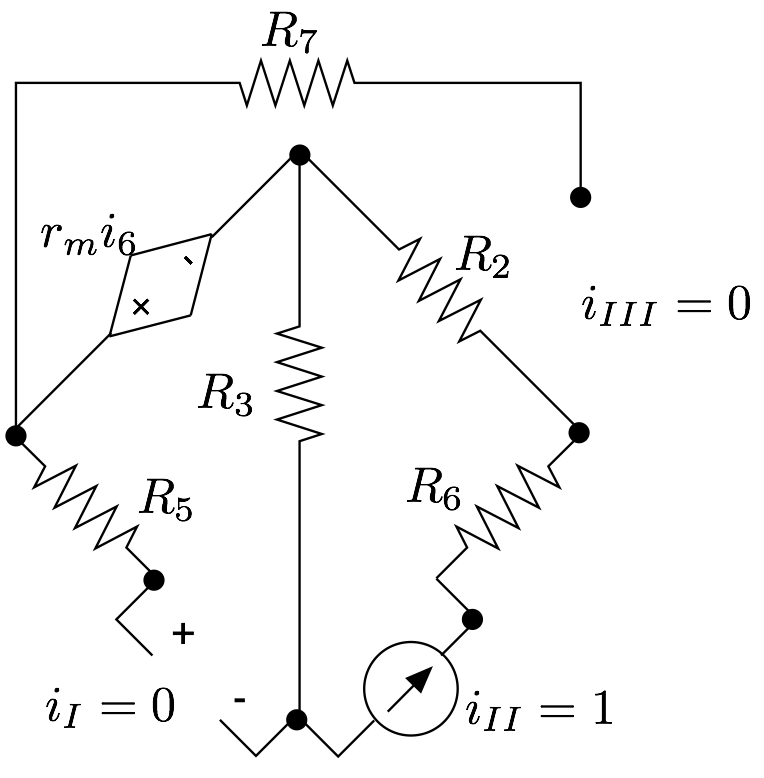
\includegraphics[width=0.4\linewidth]{figs/methodes-generales/ex_exp_MM_2}
	\end{center}
	on a $i_5=0$, $i_6=1$, et $R_{12}=v_{I}= R_3+r_m$.
	
	Finalement, pour $R_{13}=v_{I}|_{i_{III}=1,i_{I}=i_{II}=0}$
	\begin{center}
		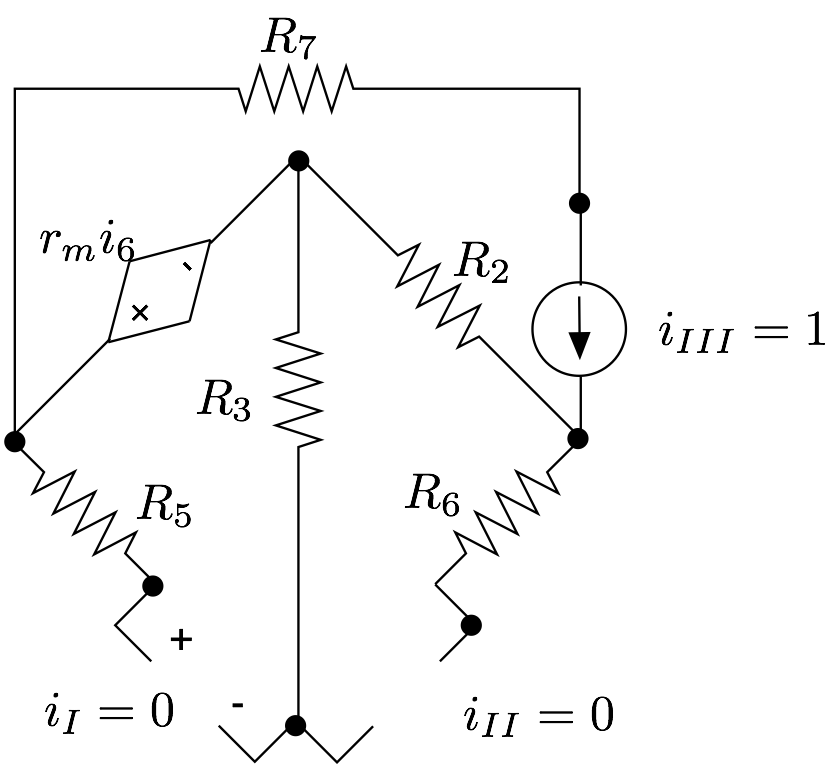
\includegraphics[width=0.4\linewidth]{figs/methodes-generales/ex_exp_MM_3}
	\end{center}
	on a $i_6=0$, et $R_{13} = v_{I}= 0$.
\end{testexample}


\subsection{Gestion des sources dépendantes de type CVT}
L'exemple de la section précédente nous a montré comment gérer un source de type CVT. On peut également les traiter avec la méthode de base, lors de la construction de la matrice $\mathbf{R}_B$, la matrice ${\bf B}$ étant indépendante de la nature des éléments qui constituent les branches. 

\begin{testexample}
	Soit le circuit de la figure suivante, comportant une source CVT :
	\begin{center}
		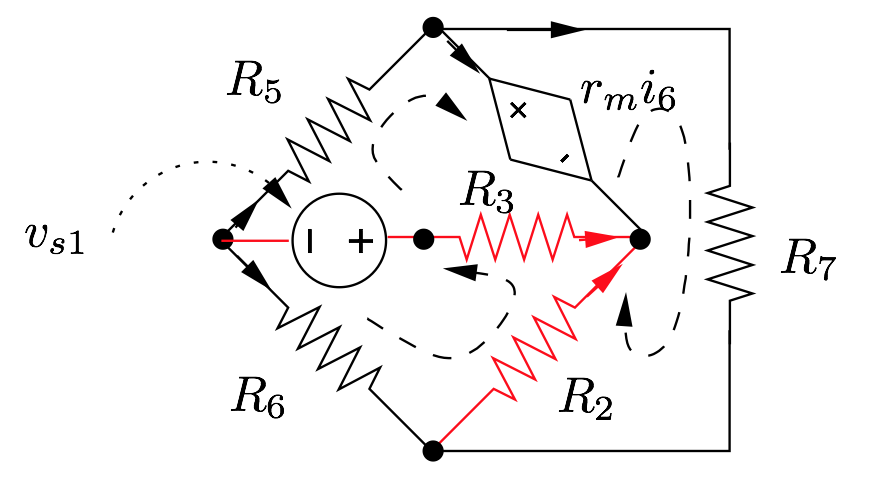
\includegraphics[width=0.5\linewidth]{figs/methodes-generales/ex_exp_MM_0}
	\end{center}
	\[{\bf R}_B=
	\left[
	\begin{array}{cccccc}
	0 & 0 & 0 & 0 & r_m & 0\\
	0 & R_2 & 0 & 0 & 0 & 0 \\
	0 & 0 & R_3 & 0 & 0 & 0\\
	0 & 0 & 0 & R_5 & 0 & 0\\
	0 & 0 & 0 & 0 & R_6 & 0\\
	0 & 0 & 0 & 0 & 0 & R_7
	\end{array}\right]\]
	
	\[{\bf R}_M={\bf B}{\bf R}_B{\bf B}^T= 
	\left[
	\begin{array}{ccc}
	R_3+R_5 & R_3+r_m & 0 \\
	R_3 & R_2+R_3+R_6 & R_2 \\
	0 & R_2-r_m & R_2+R_7
	\end{array}\right]\]
	
	${\bf R}_B$ et  ${\bf R}_M$ ne sont plus des matrices symétriques.
\end{testexample}

Par contre,  ${\bf R}_M$ ne peut plus être déterminée par inspection, ou en tous les cas pas totalement.

\subsection{Gestion des sources indépendantes de tension}

Pour gérer les sources indépendantes de courant, on peut transformer le circuit comme suit : 
\begin{itemize}
	\item pour une source en parallèle avec une résistance : transformer la source de
	courant en une source de tension  équivalente
	\item pour source seule dans une branche : transformer le circuit comme indiqué à la Figure~\ref{fig:transformation_SIT}.
\end{itemize}
\begin{figure}[htb]
	\centering
	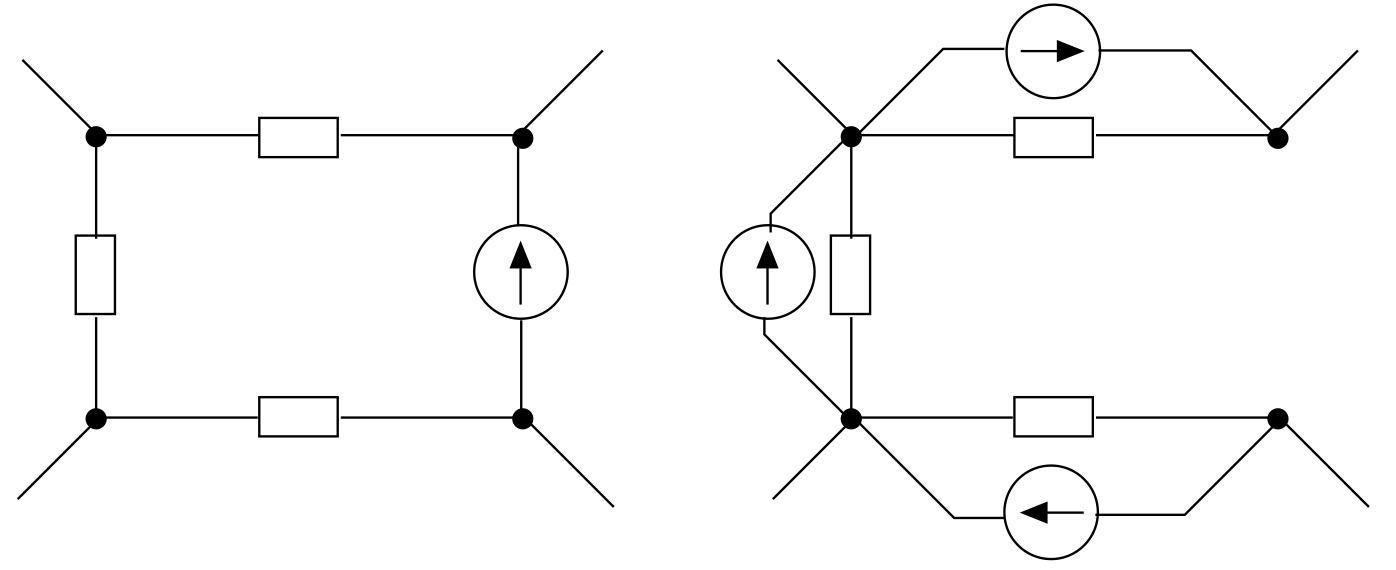
\includegraphics[width=0.95\linewidth]{figs/methodes-generales/transformation_SIT}
	\caption{Gestion des sources indépendantes de courant dans la méthode des mailles.}
	\label{fig:transformation_SIT}
\end{figure}

On vérifie que dans le reste du circuit, les lois de Kirchhoff sont inchangées. La branche dans laquelle se trouve la source de courant ne doit pas être couplée avec le reste du circuit (par une source commandée, par exemple).

\subsection{Généralisation du Théorème de Thévenin à plusieurs accès}
Considérons le schéma équivalent du circuit déduit de la méthode des mailles (Figure~\ref{fig:theveninMM}), avec $M=n-(n-1)$ accès.
Les relations $u-i$ pour les $M$ accès:
\[{\bf u}=-{\bf v}_{sM}+{\bf R}_M{\bf i}_M\]
ou encore
\[{\bf u}=-{\bf v}_{sM}+{\bf R}_M{\bf i}\]
On en déduit le schéma équivalent de Thévenin à $M$ accès par simple identification :
\[ {\bf v}_{th} = - {\bf v}_{sM}\,\, , \quad \quad {\bf R}_{Th}={\bf R}_{M}\]
\begin{figure}[htb]
	\centering
	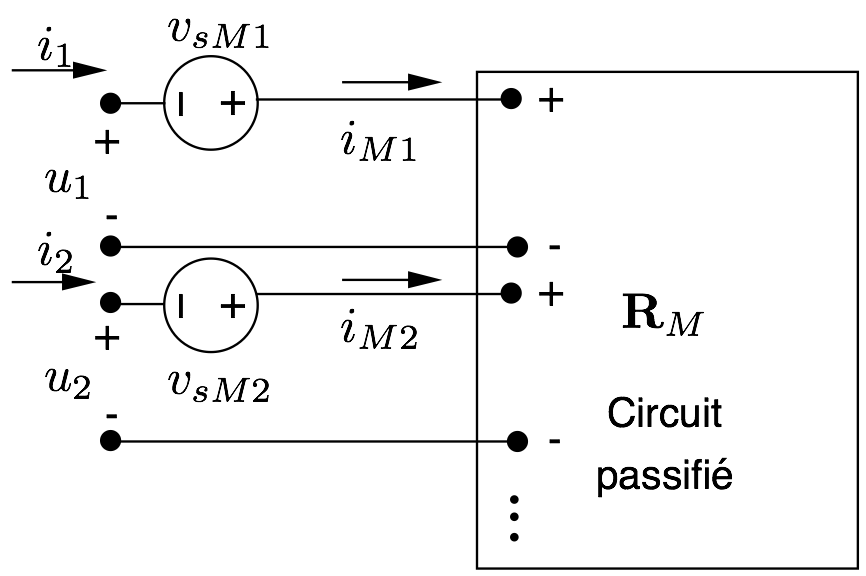
\includegraphics[width=0.7\linewidth]{figs/methodes-generales/thevenin}
	\caption{Généralisation du Théorème de Thévenin à plusieurs accès.}
	\label{fig:theveninMM}
\end{figure}

\subsection{Réduction du nombre d'accès}
On cherche à obtenir un schéma équivalent de Thévenin à $a$ accès (intéressants), avec $a<M$.
Les $M-a$ accès inintéressants sont court-circuités (ce qui ne dénature pas la topologie du circuit) : 
\[v_{a+1},\ldots,v_N=0\]
\begin{figure}[htb]
	\centering
	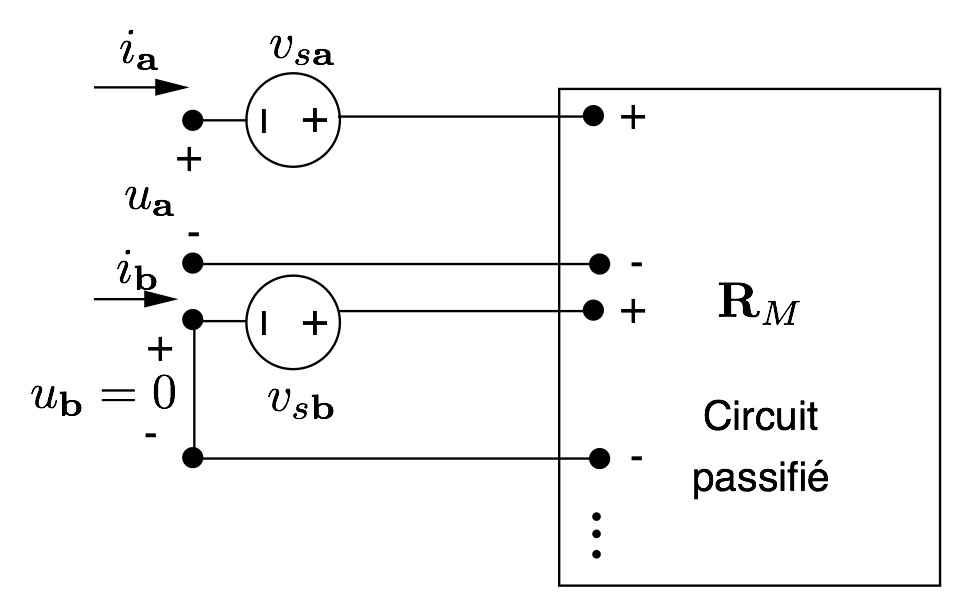
\includegraphics[width=0.7\linewidth]{figs/methodes-generales/reduction_MM}
	\caption{Illustration de la réduction du nombre d'accès.}
	\label{fig:reduction_MM}
\end{figure}
Utilisons les indices $\mathbf{a}$ et $\mathbf{b}$ pour partitionner les vecteurs en parties intéressantes et non-intéressantes. Les relations $u-i$ de la méthode des mailles deviennent : 
{\small
	\[\left[
	\begin{array}{c}
	{\bf u}_{\bf a}\\
	{\bf u}_{\bf b}
	\end{array}\right]=
	- \left[
	\begin{array}{c}
	{\bf v}_{s{\bf a}}\\
	{\bf v}_{s{\bf b}}
	\end{array}\right] + 
	\left[
	\begin{array}{cc}
	{\bf R}_{\bf a,a}& {\bf R}_{\bf a,b}\\
	{\bf R}_{\bf b,a}& {\bf R}_{\bf b,b}
	\end{array}\right]
	\left[
	\begin{array}{c}
	{\bf i}_{\bf a}\\
	{\bf i}_{\bf b}
	\end{array}\right]\]
	
	\[
	{\bf u}_{\bf b}=0 =-{\bf v}_{s{\bf b}}+{\bf R}_{\bf b,a}{\bf i}_{\bf a}+{\bf
		R}_{\bf b,b}{\bf i}_{\bf b} \rightarrow 
	{\bf i}_{\bf b}={\bf R}_{\bf b,b}^{-1}({\bf v}_{s{\bf b}}-{\bf R}_{\bf
		b,a}{\bf
		i}_{\bf a})\]
	
	\[{\bf u}_{\bf a}=(-{\bf v}_{s{\bf a}}+{\bf R}_{\bf a,b}{\bf R}_{\bf b,b}^{-1}{\bf
		v}_{s{\bf b}})
	+({\bf R}_{\bf a,a}-{\bf R}_{\bf a,b}{\bf R}_{\bf b,b}^{-1}{\bf
		R}_{\bf b,a}){\bf
		i}_{\bf a}\]
	
	Finalement :
	\[ {\bf u}_{\bf a}=
	{\bf v}_{Th}+{\bf R}_{Th}{\bf i}_{\bf a}\]}
on a 
\begin{itemize}
	\item le vecteur des sources équivalentes de Thévenin :
	\[{\bf v}_{Th}=-{\bf v}_{s{\bf a}}+{\bf R}_{\bf a,b}{\bf R}_{\bf b,b}^{-1}{\bf
		v}_{s{\bf b}}\]
	c'est le vecteur des tensions  aux bornes des accès à vide
	(${\bf i}_{\bf a}={\bf 0}$)
	\item la matrice de résistances de Thévenin, 
	matrice de résistances ``réduite'' aux accès :
	\[{\bf R}_{Th}={\bf R}_{\bf a,a}-{\bf R}_{\bf a,b}{\bf R}_{\bf b,b}^{-1}{\bf
		R}_{\bf b,a}\]
	qui peut être déterminée par expérimentation, mais jamais par inspection.
\end{itemize}

\section{Identification des paramètres d'un quadripôle}


\subsection{Objectifs de l'analyse des quadripôles}

Le quadripôle occupe une place de choix en théorie des circuits.
Que ce soit en télécommunications, en électroacoustique, en électronique ou en électrotechnique, il est
en effet couramment utilisé comme élément de liaison ; citons par exemple le quadripôle
"filtre" aux fonctions aussi multiples qu'importantes.
Lors de la conception d'un circuit électrique par exemple celui illustré à la Figure~\ref{fig:exemple}, on utilise souvent une approche modulaire. Chaque module est conçu de manière indépendante, et est caractérisé par ses relations entrées-sorties. Moyennant certaines précautions d'implémentation des modules, on évite de devoir traiter les détails internes de chacun des modules lors de la conception du système global. Cela facilite aussi le réemploi de certains modules, le partage du travail, la réparation, l'analyse de fiabilité, etc.
\begin{figure}[ht]
\centering
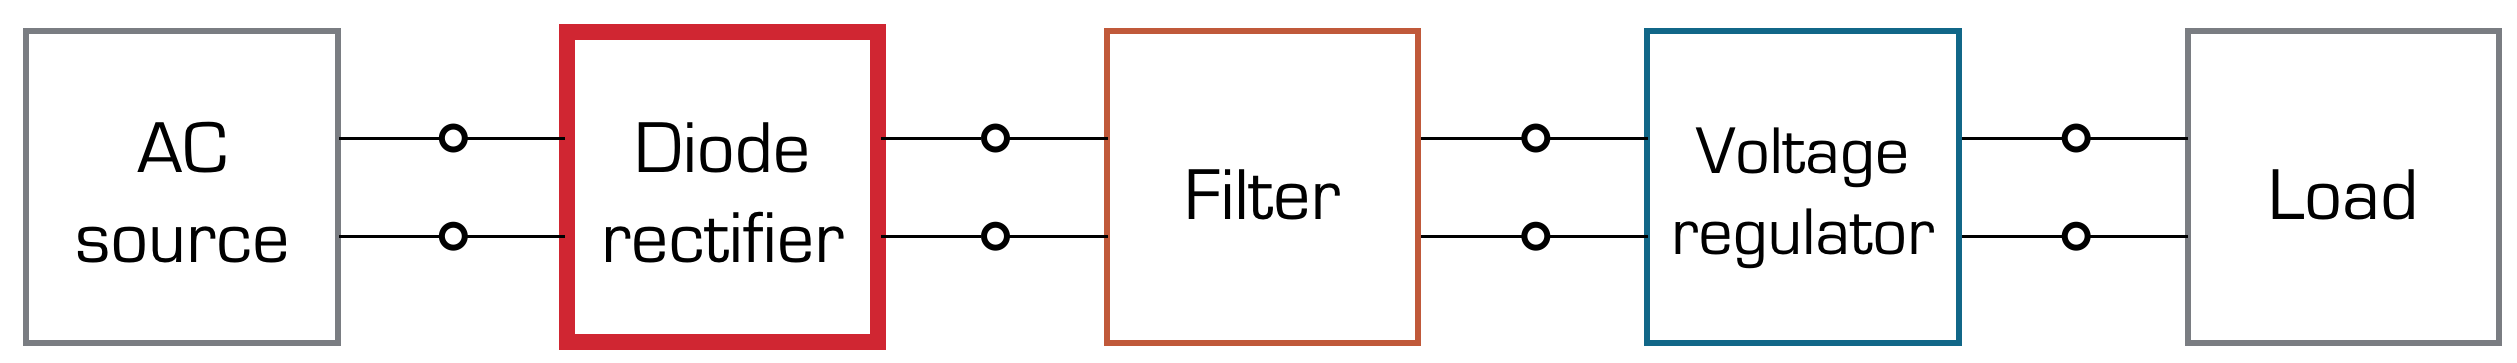
\includegraphics[width=0.95\linewidth]{figs/QP/exemple}
\caption{Exemple: vue modulaire d'une unité de conversion de puissance AC-DC.}
\label{fig:exemple}
\end{figure}

On souhaite donc caractériser les relations ``entre accès'':
\begin{align*}
f_1(u_1(t),u_2(t),i_1(t),i_2(t))& = 0\\
f_2(u_1(t),u_2(t),i_1(t),i_2(t))& = 0
\end{align*}
Par exemple, pour la source commandée de type CCT illustrée à la Figure~\ref{fig:CCT}, on a 
\begin{align*}
u_1&=0\\
i_2& =f(i_1).
\end{align*}

\begin{marginfigure}
	\centering
\begin{circuitikz}[american voltages]
	\draw (0,0) coordinate (A1) 
	to [short, *-] ++(1,0)
	to [short] ++(0,2)
	to [short, -*, i<=$i_1$] ++(-1,0) coordinate (A1');
	\draw (3.5,2) coordinate (A2') 
	to [short, *-, i=$i_2$] ++(-1,0)
	to [american controlled current source, l_=$f(i_1)$] ++(0,-2)
	to [short, -*] ++(1,0) coordinate (A2);
	\draw (A1') to[open,v=$u_1$] (A1);
	\draw (A2') to[open,v^=$u_2$] (A2);
\end{circuitikz}
\caption{Exemple de quadripôle avec une source de type CCT.}\label{fig:CCT}
\end{marginfigure}
De plus, 
\begin{itemize}
	\item Si le quadripôle est linéaire : $f(i_1)=\beta(t)\, i_1$
	\item si de plus il est invariant : $f(i_1)=\beta \, i_1$
\end{itemize}


Si un quadripôle n'est pas exclusivement résistif (R, L, C, ...), sa caractérisation est parfois très difficile sauf s'il est composé d' éléments linéaires et invariants, auquel cas on peut faire recours à l'approche fréquentielle.
Par exemple, en régime sinusoïdal établi, on aura recours aux phaseurs, $Z$ et $Y$.

\subsection{Caractérisation}
Il existe 6 manières de caractériser un quadripôle. Elles dépendent des combinaisons possibles entre variables. 
Chaque manière est caractérisée par une matrice $2\times2$ exprimant les relations entre $u_1,\, i_1,\, u_2, \, i_2$.

\begin{center}
	\begin{tabular}{l l | c}
		Exprimer & en fonction & Matrice \\
		\hline
		les tensions & des courants & $\mathbf{Z}$ \\
		les courants & des tensions & $\mathbf{Y}$ \\
		les grandeurs du primaire & des grandeurs du secondaire & $\mathbf{T}$ \\
		les grandeurs du secondaire & des grandeurs du primaire & $\mathbf{T}_-$ \\
		$(\bar{U}_1, \bar{I}_2)$ & de $(\bar{U}_2, \bar{I}_1)$& $\mathbf{H}$ \\
		$(\bar{U}_2, \bar{I}_1)$ & de $(\bar{U}_1, \bar{I}_2)$& $\mathbf{G}$
	\end{tabular}
\end{center}	
On choisit l'une ou l'autre en fonction de l'application. L'objectif de ce chapitre est de montrer comment identifier les paramètres de ces matrices et de faire le lien avec les sections précédentes.\mytodo{Lien quadripôles - méthodes générales d'analyse.}

\subsection{Matrice d'impédances $\mathbf{Z}(j\omega)$}%
\[
{\bf U}=\left(
\begin{array}{l}
\bar{U}_1\\
\bar{U}_2
\end{array} \right)
= \left(
\begin{array}{cc}
Z_{11}(j\omega)  &Z_{12}(j\omega)\\
Z_{21}(j\omega)  &Z_{22}(j\omega)
\end{array} \right)\left(
\begin{array}{l}
\bar{I}_1\\
\bar{I}_2
\end{array} \right)={\bf Z}(j\omega){\bf I}\]
${\bf Z}(j\omega)$ est la matrice d'impédances du circuit réduite à ses accès $11'$
et $22'$.
Les éléments de ${\bf Z}$ sont obtenus par essais à vide :
\begin{xalignat*}{2}
	Z_{11} &= \frac{\bar{U}_1}{\bar{I}_1}|_{\bar{I}_2=0} & Z_{22} &= \frac{\bar{U}_2}{\bar{I}_2}|_{\bar{I}_1=0}\\
	Z_{21} &= \frac{\bar{U}_2}{\bar{I}_1}|_{\bar{I}_2=0} & Z_{12} &= \frac{\bar{U}_1}{\bar{I}_2}|_{\bar{I}_1=0}
\end{xalignat*}


%--------------------------------------------------------------------------------

\paragraph{Cas du quadripôle \textbf{réciproque}.}%
La matrice ${\bf Z}(j\omega)$ d'un quadripôle réciproque est symétrique : $$Z_{12}(j\omega)=Z_{21}(j\omega)$$

Car, comme illustré à la Figure~\ref{fig:identificationZ}, 
\[Z_{21} = \bar{U}_2|_{\bar{I}_1=1;\bar{I}_2=0}\]
\[Z_{12} = \bar{U}_1|_{\bar{I}_1=0;\bar{I}_2=1}\]
Et d'après la condition 2 de la propriété de réciprocité : $\bar{U}_1=Z_{12}=\bar{U}_2=Z_{21}$.
\begin{figure*}[htb]
	\centering
\begin{circuitikz}[american voltages]% or tikzpicture
	\tikzset{quad/.style={draw, thick, minimum height=2.5cm, minimum width=2cm}}
	\node[quad] (A) at (0,0) {};
	\draw ($(A.north west)!.5!(A.west)$) to[short] ++(-.5,0) to[short,-*] ++(-0.2,0) coordinate (A1)
	($(A.south west)!.5!(A.west)$) to[short] ++(-.5,0) to[short,-*] ++(-0.2,0) coordinate (A1')
	($(A.north east)!.5!(A.east)$) to[short, i<=$i_2^a$] ++(.5,0) to[short,-*] ++(0.2,0) coordinate (A2)
	($(A.south east)!.5!(A.east)$) to[short] ++(.5,0) to[short,-*] ++(0.2,0) coordinate (A2');
	\draw (A1') to[american current source, l=$1A$] (A1);
	\draw (A2) to[open, v^=$\bar{U}_{2}$] (A2');
\end{circuitikz} \hspace{1cm} %
\begin{circuitikz}[american voltages]% or tikzpicture
	\tikzset{quad/.style={draw, thick, minimum height=2.5cm, minimum width=2cm}}
	\node[quad] (A) at (0,0) {};
	\draw ($(A.north west)!.5!(A.west)$) to[short, i<_=$i_1^b$] ++(-.5,0) to[short,-*] ++(-0.2,0) coordinate (A1)
	($(A.south west)!.5!(A.west)$) to[short] ++(-.5,0) to[short,-*] ++(-0.2,0) coordinate (A1')
	($(A.north east)!.5!(A.east)$) to[short] ++(.5,0) to[short,-*] ++(0.2,0) coordinate (A2)
	($(A.south east)!.5!(A.east)$) to[short] ++(.5,0) to[short,-*] ++(0.2,0) coordinate (A2');
	\draw (A2') to[american current source, l_=$1A$] (A2);
	\draw (A1) to[open, v=$\bar{U}_{1}$] (A1');
\end{circuitikz}
\caption{Indentification de ${\bf Z}$.} \label{fig:identificationZ}
\end{figure*}

\paragraph{Propriété des "quadripôles RLC".}
Tout quadripôle ne comportant que des éléments R, L, C classiques linéaires et invariants \textbf{est réciproque}.
\footnote{Un quadripôle comportant des sources commandées ou des AO peut ne pas être réciproque.}

\paragraph{Cas du quadripôle \textbf{symétrique}.}%
Connectons aux deux accès deux sources de courant.\\[5mm]
\begin{center}
\begin{circuitikz}[american voltages]% or tikzpicture
	\tikzset{quad/.style={draw, thick, minimum height=2.5cm, minimum width=2cm}}
	\node[quad] (A) at (0,0) {};
	\draw ($(A.north west)!.5!(A.west)$) node[right] {$1$} to[short] ++(-.5,0) to[short,-*] ++(-0.2,0) coordinate (A1)
	($(A.south west)!.5!(A.west)$) node[right] {$1'$} to[short] ++(-.5,0) to[short,-*] ++(-0.2,0) coordinate (A1')
	($(A.north east)!.5!(A.east)$) node[left] {$2$} to[short] ++(.5,0) to[short,-*] ++(0.2,0) coordinate (A2)
	($(A.south east)!.5!(A.east)$) node[left] {$2'$} to[short] ++(.5,0) to[short,-*] ++(0.2,0) coordinate (A2');
	\draw (A1') to[american current source, l=$\bar{I}_1$] (A1);
	\draw (A2') to[american current source, l_=$\bar{I}_2$] (A2);
\end{circuitikz}
\end{center}
\[\bar{U}_1=Z_{11}\bar{I}_1 + Z_{12} \bar{I}_2\]
Inversons les accès en retournant le quadripôle.
\begin{center}
\begin{circuitikz}[american voltages]% or tikzpicture
	\tikzset{quad/.style={draw, thick, minimum height=2.5cm, minimum width=2cm}}
	\node[quad] (A) at (0,0) {};
	\draw ($(A.north west)!.5!(A.west)$) node[right] {\alert{$2$}} to[short] ++(-.5,0) to[short,-*] ++(-0.2,0) coordinate (A1)
	($(A.south west)!.5!(A.west)$) node[right] {\alert{$2'$}} to[short] ++(-.5,0) to[short,-*] ++(-0.2,0) coordinate (A1')
	($(A.north east)!.5!(A.east)$) node[left] {\alert{$1$}} to[short] ++(.5,0) to[short,-*] ++(0.2,0) coordinate (A2)
	($(A.south east)!.5!(A.east)$) node[left] {\alert{$1'$}} to[short] ++(.5,0) to[short,-*] ++(0.2,0) coordinate (A2');
	\draw (A1') to[american current source, l=$\bar{I}_1$]  (A1);
	\draw (A2') to[american current source, l_=$\bar{I}_2$] (A2);
\end{circuitikz}
\end{center}
\[\bar{U}_2=Z_{22}\bar{I}_1 + Z_{21}\bar{I}_2\]
Si le quadripôle est symétrique, il faut
\[\bar{U}_1=\bar{U}_2 \quad \forall \bar{I}_1, \, \bar{I}_2 \quad \Rightarrow Z_{11}=Z_{22} 
\quad \text{et} \quad Z_{12}=Z_{21}\]
Donc $\mathbf{Z}(j\omega)$ doit être symétrique et telle que $Z_{11}=Z_{22}$.


%--------------------------------------------------------------------------------

\subsection{Matrice d'admittances}%
\[
{\bf I}=\left(
\begin{array}{l}
\bar{I}_1\\
\bar{I}_2
\end{array} \right)
= \left(
\begin{array}{cc}
Y_{11}(j\omega)  &Y_{12}(j\omega)\\
Y_{21}(j\omega)  &Y_{22}(j\omega)
\end{array} \right)\left(
\begin{array}{l}
\bar{U}_1\\
\bar{U}_2
\end{array} \right)={\bf Y}(s){\bf U}(s)\]
${\bf Y}(s)$ = matrice d'admittances du circuit réduite à ses accès 11'
et 22'.
Les éléments de ${\bf Y}$ sont obtenus par essais en court-circuit :
\begin{xalignat*}{2}
	Y_{11} &= \frac{\bar{I}_1}{\bar{U}_1}|_{\bar{U}_2=0} & Y_{22} &= \frac{\bar{I}_2}{\bar{U}_2}|_{\bar{U}_1=0}\\
	Y_{21} &= \frac{\bar{I}_2}{\bar{U}_1}|_{\bar{U}_2=0} & Y_{12} &= \frac{\bar{I}_1}{\bar{U}_2}|_{\bar{U}_1=0}
\end{xalignat*}
\begin{itemize}
	\item Quadripôle \textbf{réciproque} : $Y_{12}(j\omega)=Y_{21}(j\omega)$ (condition 1).\\
	\item Quadripôle \textbf{symétrique} :  $Y_{11}(j\omega)=Y_{22}(j\omega)$ et $Y_{12}(j\omega)=Y_{21}(j\omega)$.
\end{itemize}


%--------------------------------------------------------------------------------

\subsection{Matrice de transfert directe $\mathbf{T}(j\omega)$}%
Elle relie les grandeurs d'un accès à celles de l'autre accès :
\[
\left(
\begin{array}{l}
\bar{U}_1\\
\bar{I}_1
\end{array} \right)
= \left(
\begin{array}{cc}
A(j\omega) & B(j\omega)\\
C(j\omega)  &D(j\omega)
\end{array} \right)\left(
\begin{array}{l}
\bar{U}_2\\
\bar{I}^{'}_2
\end{array} \right)={\bf T}(j\omega)
\left(
\begin{array}{l}
\bar{U}_2\\
\bar{I}^{'}_2
\end{array} \right)
\]
Les éléments de ${\bf T}$ sont obtenus par des essais à vide et en court-circuit :
\begin{minipage}[c]{6cm}
	\begin{xalignat*}{2}
		A &= \left.\frac{\bar{U}_1}{\bar{U}_2}\right|_{\bar{I}^{'}_2=0} & B &=\left.\frac{\bar{U}_1}{\bar{I}^{'}_2}\right|_{\bar{U}_2=0}\\
		C &=  \left.\frac{\bar{I}_1}{\bar{U}_2}\right|_{\bar{I}^{'}_2=0} & D &= \left.\frac{\bar{I}_1}{\bar{I}^{'}_2}\right|_{\bar{U}_2=0}
	\end{xalignat*}
\end{minipage}
\begin{minipage}[c]{6cm}
	\begin{center}
		%TODO \begin{tikzpicture}[y=-1cm]
\sf
\path (5.22889,6.31333) node[text=black,anchor=base] {$I^{'}_{2}$};
\draw[arrows=-triangle 45,black] (4.93556,5.92889) -- (5.59111,5.92889);
\path (5.38889,5.51111) node[text=black,anchor=base] {$I_2$};
\path (6.05556,6.46667) node[text=black,anchor=base west] {$U_2$};
\path (1.88889,5.45556) node[text=black,anchor=base] {$I_1$};
\path (1.02222,6.44444) node[text=black,anchor=base east] {$U_1$};
\path (6.1,5.85556) node[text=black,anchor=base] {+};
\path (6.04444,6.91111) node[text=black,anchor=base] {-};
\path (1.08889,6.95556) node[text=black,anchor=base] {-};
\path (1.12222,5.84444) node[text=black,anchor=base] {+};
\draw[arrows=-triangle 45,black] (5.56667,5.65556) -- (4.91111,5.65556);
\draw[black] (4.66667,5.77778) -- (5.74889,5.77778);
\draw[black] (4.65556,6.86667) -- (5.73778,6.86667);
\draw[arrows=-triangle 45,black] (1.62222,5.63333) -- (2.27778,5.63333);
\draw[black] (1.40667,5.77778) -- (2.48889,5.77778);
\draw[black] (1.40667,6.85556) -- (2.48889,6.85556);
\draw[black] (2.5,5.6) rectangle (4.65778,7.05556);
\filldraw[black] (5.75556,6.86667) ellipse (0.06667cm and 0.06667cm);
\filldraw[black] (5.76667,5.77778) ellipse (0.06667cm and 0.06667cm);
\filldraw[black] (1.38889,6.86667) ellipse (0.06667cm and 0.06667cm);
\filldraw[black] (1.38889,5.75556) ellipse (0.06667cm and 0.06667cm);

\end{tikzpicture}%

%% Configure (x)emacs for this file ...
%% Local Variables:
%% mode: latex
%% End:
	\end{center}
\end{minipage}


%--------------------------------------------------------------------------------

\paragraph{Relations avec les éléments des matrices ${\bf Z}$ et ${\bf Y}$.}%
\begin{xalignat*}{2}
	A & = \frac{Z_{11}}{Z_{21}} & C & = \frac{1}{Z_{21}}\\
	B & = -\frac{1}{Y_{21}} & D & = -\frac{Y_{11}}{Y_{21}}
\end{xalignat*}
Comme ${\bf Z}={\bf Y}^{-1}$ et ${\bf Y}={\bf Z}^{-1}$
\begin{xalignat*}{2}
	A& = -\frac{Y_{22}}{Y_{21}}  & C & = -\frac{\text{det}\,{\bf Y}}{Y_{21}} \\
	B& = \frac{\text{det}\,{\bf Z}}{Z_{21}}  & D & = \frac{Z_{22}}{Z_{21}}
\end{xalignat*}


\begin{itemize}
	\item Quadripôle \textbf{réciproque} : on vérifie $\text{det}\, {\bf T}=AD-BC=1$
	\item Quadripôle \textbf{symétrique} : en plus $A=D$
\end{itemize}


%--------------------------------------------------------------------------------

\subsection{Matrice de transfert inverse $\mathbf{T}_-(j\omega)$}%
\[
\left(
\begin{array}{l}
\bar{U}_2\\
\bar{I}_2
\end{array} \right)
= \left(
\begin{array}{cc}
A^{'}(j\omega) & B^{'}(j\omega)\\
C^{'}(j\omega)  &D^{'}(j\omega)
\end{array} \right)\left(
\begin{array}{l}
\bar{U}_1\\
\bar{I}^{'}_1
\end{array} \right)={\bf T}_{-}(j\omega)
\left(
\begin{array}{l}
\bar{U}_1\\
\bar{I}^{'}_1
\end{array} \right)
\]

\begin{center}
	%TODO \begin{tikzpicture}[y=-1cm]
\sf
\path (6.05556,6.46667) node[text=black,anchor=base west] {$\bar{U}_2$};
\path (5.38889,5.51111) node[text=black,anchor=base] {$\bar{I}_2$};
\path (1.88889,5.45556) node[text=black,anchor=base] {$\bar{I}_1$};
\path (1.95778,6.34444) node[text=black,anchor=base] {$\bar{I}^{'}_{1}$};
\path (1.02222,6.44444) node[text=black,anchor=base east] {$\bar{U}_1$};
\filldraw[black] (1.38889,5.75556) ellipse (0.06667cm and 0.06667cm);
\filldraw[black] (1.38889,6.86667) ellipse (0.06667cm and 0.06667cm);
\filldraw[black] (5.76667,5.77778) ellipse (0.06667cm and 0.06667cm);
\filldraw[black] (5.75556,6.86667) ellipse (0.06667cm and 0.06667cm);
\draw[black] (2.5,5.6) rectangle (4.65778,7.05556);
\draw[black] (1.40667,6.85556) -- (2.48889,6.85556);
\draw[black] (1.40667,5.77778) -- (2.48889,5.77778);
\draw[arrows=-triangle 45,black] (1.62222,5.63333) -- (2.27778,5.63333);
\draw[black] (4.65556,6.86667) -- (5.73778,6.86667);
\draw[black] (4.66667,5.77778) -- (5.74889,5.77778);
\draw[arrows=-triangle 45,black] (5.56667,5.65556) -- (4.91111,5.65556);
\path (1.12222,5.84444) node[text=black,anchor=base] {+};
\path (1.08889,6.95556) node[text=black,anchor=base] {-};
\path (6.04444,6.91111) node[text=black,anchor=base] {-};
\path (6.1,5.85556) node[text=black,anchor=base] {+};
\draw[arrows=-triangle 45,black] (2.26,5.92889) -- (1.60444,5.92889);

\end{tikzpicture}%

%% Configure (x)emacs for this file ...
%% Local Variables:
%% mode: latex
%% End:
\end{center}


%--------------------------------------------------------------------------------

\paragraph{Relation avec la matrice ${\bf T}$.}%


De la définition de ${\bf T}$
\[
\begin{pmatrix}
\bar{U}_2\\
\bar{I}_2^{'}
\end{pmatrix} = \frac{1}{\text{det}\, {\bf T}}
\begin{pmatrix}
D & -B\\
-C & A
\end{pmatrix}
\begin{pmatrix}
\bar{U}_1\\\bar{I}_1
\end{pmatrix}\]
De là:
\[
\begin{pmatrix}
\bar{U}_2\\
\bar{I}_2
\end{pmatrix} = \frac{1}{\text{det}\, {\bf T}}
\begin{pmatrix}
D & B\\
C & A
\end{pmatrix}
\begin{pmatrix}
\bar{U}_1\\\bar{I}_1^{'}
\end{pmatrix}\]


\begin{itemize}
	\item Quadripôle \textbf{réciproque} : $\text{det}\, {\bf T}_{-}=1$
	\item Quadripôle \textbf{symétrique} : en plus $A^{'}=D^{'} \quad \Rightarrow \quad {\bf T}={\bf T}_{-}$
\end{itemize}	


%--------------------------------------------------------------------------------

\paragraph{Remarque.}%
La matrice de transfert ${\bf T}$ est plus générale que la matrice
d'impédances ${\bf Z}$ ou la matrice d'admittances ${\bf Y}$.

Certains quadripôles possèdent une matrice ${\bf Z}$ singulière et
donc pas de matrice~${\bf Y}$  :
\begin{center}
\begin{circuitikz}[american voltages]% or tikzpicture
	\draw (0,0) coordinate (A1)
	to[short, *-*] ++(1,0) coordinate (C)
	to[short, *-*] ++(1,0) coordinate (A2);
	\draw (0,2) coordinate (A1')
	to[short, *-*, i=$\bar{I}_1$] ++(1,0) coordinate (C')
	to[short, *-*, i<=$\bar{I}_2$] ++(1,0) coordinate (A2');
	\draw (C) to[R, l=$Z$] (C');
	\draw (A1') to[open, v_=$\bar{U}_1$] (A1);
	\draw (A2') to[open, v^=$\bar{U}_2$] (A2);
\end{circuitikz}
\end{center}
\[{\bf Z} =
\begin{pmatrix}
Z & Z \\
Z & Z
\end{pmatrix} \qquad
{\bf T} = 
\begin{pmatrix}
1 & 0 \\
\frac{1}{Z} & 1 
\end{pmatrix}\]
D'autres ont une matrice ${\bf Y}$ singulière et donc pas de matrice ${\bf Z}$. 
Certains n'ont ni matrice ${\bf Z}$ ni matrice ${\bf Y}$.
Ils ont tous une matrice de transfert ${\bf T}$


%--------------------------------------------------------------------------------

\subsection{Matrices hybrides}%

Elles relient les grandeurs relatives à des accès différents et sont surtout utilisées pour les circuits électroniques.
\[
\left(
\begin{array}{l}
\bar{U}_1\\
\bar{I}_2
\end{array} \right)
={\bf H}\left(
\begin{array}{l}
\bar{I}_1\\
\bar{U}_2
\end{array} \right)
\]

\[
\left(
\begin{array}{l}
\bar{I}_1\\
\bar{U}_2
\end{array} \right)
={\bf G}\left(
\begin{array}{l}
\bar{U}_1\\
\bar{I}_2
\end{array} \right)
\]

on a évidemment 
\[{\bf G}={\bf H}^{-1}\]

\subsection{Quadripôles réciproques usuels}

\paragraph{Quadripôles en $T$ et en $\Pi$.}%
\[{\bf Z}_{T}=\left(
\begin{array}{cc}
Z_1+Z_3 & Z_3\\
Z_3 & Z_2+Z_3
\end{array}\right)\]
\begin{marginfigure}
\begin{center}
	\begin{circuitikz}[american voltages]% or tikzpicture
		\draw (0,0) coordinate (A1)
		to[short, *-*] ++(2,0) coordinate (C)
		to[short, *-*] ++(2,0) coordinate (A2);
		\draw (0,2) coordinate (A1')
		to[R, *-*, l=$Z_1$] ++(2,0) coordinate (C')
		to[R, *-*, l=$Z_2$] ++(2,0) coordinate (A2');
		\draw (C) to[R, l=$Z_3$] (C');
	\end{circuitikz}
\end{center}
\caption{$T$}
\end{marginfigure}
\mytodo{Identification des paramètres d'un quadripôles, illustrer méthode d'expérimentation.}


\[
{\bf Y}_{\pi}=\left(
\begin{array}{cc}
Y_1+Y_3 & -Y_3\\
-Y_3 & Y_2+Y_3
\end{array}\right)\]

\begin{marginfigure}
\begin{center}
	\begin{circuitikz}[american voltages]% or tikzpicture
		\draw (0,0) coordinate (A1)
		to[short, *-*] ++(1,0) coordinate (B)
		to[short, *-*] ++(2,0) coordinate (C)
		to[short, *-*] ++(1,0) coordinate (A2);
		\draw (0,2) coordinate (A1')
		to[short, *-*] ++(1,0) coordinate (B')
		to[R, *-*, l=$Y_3$] ++(2,0) coordinate (C')
		to[short, *-*] ++(1,0) coordinate (A2');
		\draw (C) to[R, l_=$Y_2$] (C');
		\draw (B) to[R, l=$Y_1$] (B');
	\end{circuitikz}
\end{center}
\caption{$\Pi$}
\end{marginfigure}


\paragraph{Quadripôle en treillis.}%
C'est un quadripôle à trois mailles indépendantes. Sa matrice d'impédances réduite aux accès 1 et 2 s'écrit
\begin{equation}
{\bf Z}=\frac{1}{\sum Z}\left(
\begin{array}{cc}
(Z_1+Z_2)(Z_3+Z_4) & Z_2Z_4-Z_1Z_3\\
Z_2Z_4-Z_1Z_3 & (Z_1+Z_4)(Z_2+Z_3) 
\end{array}\right) \label{eq:quad_treillis}
\end{equation}
Avec $\sum Z=Z_1+Z_2+Z_3+Z_4$.
\begin{figure*}
\begin{center}
	\begin{circuitikz}[american voltages]% or tikzpicture
		\draw (0,0) coordinate (A1)
		to[short, *-*] ++(1,0) coordinate (B)
		to[R, *-*, l_=$Z_3$] ++(3,0) coordinate (C)
		to[short, *-*] ++(1,0) coordinate (A2);
		\draw (0,2) coordinate (A1')
		to[short, *-*] ++(1,0) coordinate (B')
		to[R, *-*, l=$Z_1$] ++(3,0) coordinate (C')
		to[short, *-*] ++(1,0) coordinate (A2');
		\draw (C') to[R, l_=$Z_2$] (2.5,1) coordinate (X);
		\draw (X) to[R, l^=$Z_4$] (B');
		\draw (C) to[short] (X);
		\draw (B) to[short] (X);
	\end{circuitikz} \hspace{1cm}
	\begin{circuitikz}[american voltages]% or tikzpicture
		\draw (0,0) coordinate (A1)
		to[short, *-*] ++(1,0) coordinate (B)
		to[R, *-*, l_=$Z_1$] ++(3,0) coordinate (C)
		to[short, *-*] ++(1,0) coordinate (A2);
		\draw (0,2) coordinate (A1')
		to[short, *-*] ++(1,0) coordinate (B')
		to[R, *-*, l=$Z_1$] ++(3,0) coordinate (C')
		to[short, *-*] ++(1,0) coordinate (A2');
		\draw (C') to[R, l_=$Z_2$] (2.5,1) coordinate (X);
		\draw (X) to[R, l^=$Z_2$] (B');
		\draw (C) to[short] (X);
		\draw (B) to[short] (X);
	\end{circuitikz}
\end{center}
\caption{Treillis (gauche) et treillis symétrique (droite).}
\end{figure*}
Un cas particulier important est le treillis symétrique obtenu à partir du treillis général lorsque
\[Z_3=Z_1 \qquad \text{et} \qquad Z_4=Z_2\]
Sa matrice d'impédances se réduit à partir de (\ref{eq:quad_treillis}) ou plus simplement par des essais à vide et en court-circuit.
\[{\bf Z}=\left(
\begin{array}{cc}
\frac{Z_1+Z_2}{2} & \frac{Z_2-Z_1}{2}\\
\frac{Z_2-Z_1}{2} & \frac{Z_1+Z_2}{2}
\end{array}\right)\]


\subsection{Sources commandées}

Une source commandée est en réalité un quadripôle unidirectionnel, non autonome et actif ; un
de ses accès est celui qui exerce la commande (accès de commande), l'autre est l'accès
commandé. On distingue les quatre types de sources commandées idéales décrites ci-dessous. Un implémentation de chacun de ces quadripôles est explicitée à la Section~\ref{sec:XXT}.

\paragraph{VVT.}
\begin{center}
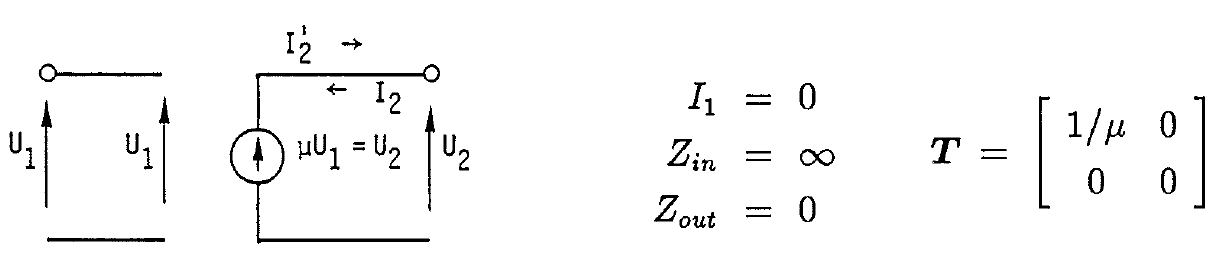
\includegraphics[width=0.9\linewidth]{figs/QP/QP_VVT}
\end{center}

\paragraph{CCT.}
\begin{center}
	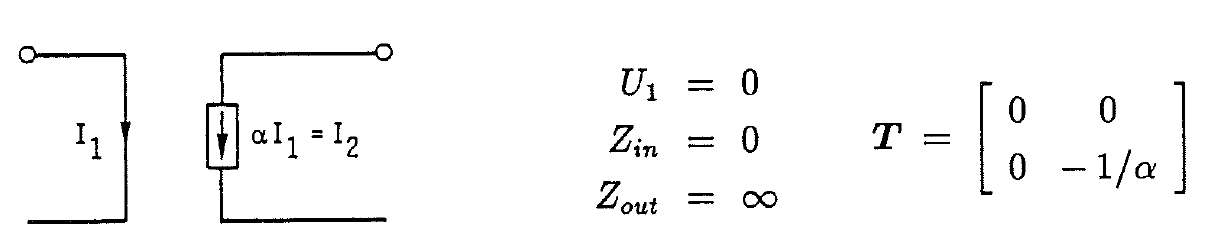
\includegraphics[width=0.9\linewidth]{figs/QP/QP_CCT}
\end{center}

\paragraph{CVT.}
\begin{center}
	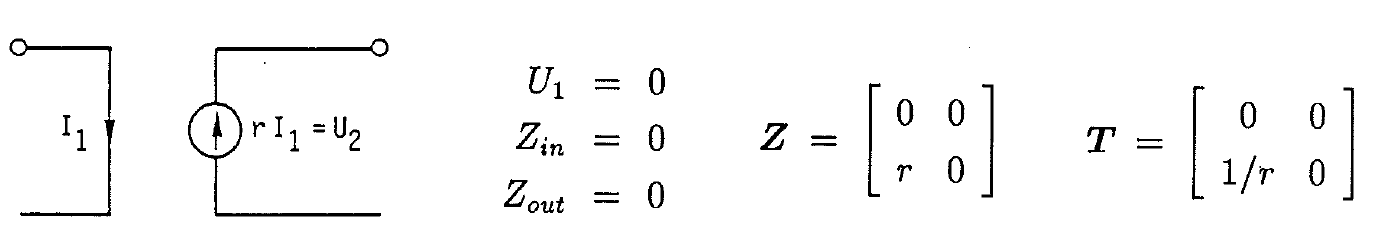
\includegraphics[width=0.9\linewidth]{figs/QP/QP_CVT}
\end{center}

\paragraph{VCT.}
\begin{center}
	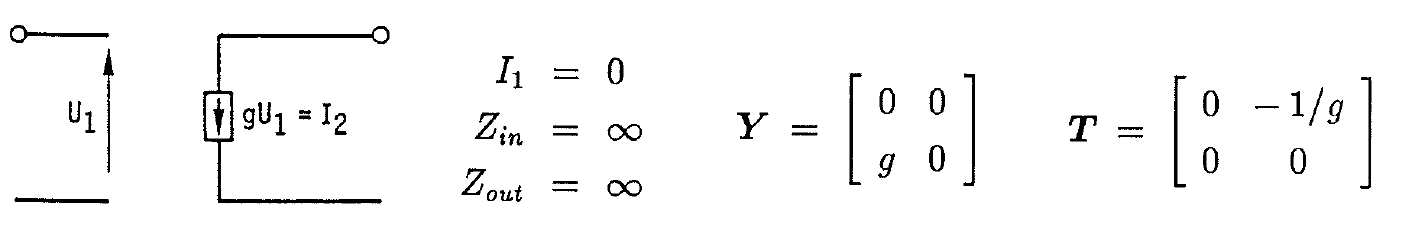
\includegraphics[width=0.9\linewidth]{figs/QP/QP_VCT}
\end{center}



\subsection{Associations de quadripôles}

\paragraph{Association en série.}%
Soient deux quadripôles $Q_a$, $Q_b$ et respectivement $\mathbf{Z}_a$, $\mathbf{Z}_b$ leurs matrices d'impédances
aux accès. Associons-les en série et recherchons la matrice $\mathbf{Z}$ du quadripôle résultant (Figure~\ref{fig:quad_serie}).

On voit ainsi que la matrice d'impédances du quadripôle résultant de l'association
de deux quadripôles en série est égale à la somme des matrices d'impédances des deux
quadripôles pris séparément:
\begin{align}
{\bf I}^{a}  &= {\bf I}^{b} = {\bf I}\notag\\
{\bf U} &={\bf U}^{a}+{\bf U}^{b}={\bf Z}^{a} {\bf I}^{a} + {\bf Z}^{b}
{\bf I}^{b}= {\bf Z}\, {\bf I}\notag\\
{\bf Z} &={\bf Z}^{a}+{\bf Z}^{b}\label{eq:quad_serie}
\end{align}
\begin{marginfigure}
	\centering
	\begin{circuitikz}[american voltages]% or tikzpicture
		\tikzset{quad/.style={draw, thick, minimum height=2.5cm, minimum width=2cm}}
		\node[quad] (A) at (0,0) {$Q^a$};
		\draw ($(A.north west)!.5!(A.west)$) node[right] {$1$} to[short, i<=$\bar{I}_1^a$] ++(-.5,0) to[short,-*] ++(-0.2,0) coordinate (A1)
		($(A.south west)!.5!(A.west)$) node[right] {$1'$} to[short, i=$\bar{I}_1^a$] ++(-.5,0) to[short,-*] ++(-0.2,0) coordinate (A1')
		($(A.north east)!.5!(A.east)$) node[left] {$2$} to[short, i<=$\bar{I}_2^a$] ++(.5,0) to[short,-*] ++(0.2,0) coordinate (A2)
		($(A.south east)!.5!(A.east)$) node[left] {$2'$} to[short, i=$\bar{I}_2^a$] ++(.5,0) to[short,-*] ++(0.2,0) coordinate (A2');
		\node[quad] (B) at (0,-3) {$Q^b$};
		\draw ($(B.north west)!.5!(B.west)$) node[right] {$1$} to[short, i<=$\bar{I}_1^b$] ++(-.5,0) to[short,-*] ++(-0.2,0) coordinate (B1)
		($(B.south west)!.5!(B.west)$) node[right] {$1'$} to[short, i=$\bar{I}_1^b$] ++(-.5,0) to[short,-*] ++(-0.2,0) coordinate (B1')
		($(B.north east)!.5!(B.east)$) node[left] {$2$} to[short, i<=$\bar{I}_2^b$] ++(.5,0) to[short,-*] ++(0.2,0) coordinate (B2)
		($(B.south east)!.5!(B.east)$) node[left] {$2'$} to[short, i=$\bar{I}_2^b$] ++(.5,0) to[short,-*] ++(0.2,0) coordinate (B2');
		\draw[color=myRed] (A1') to[short] (B1);
		\draw[color=myRed] (A2') to[short] (B2);
	\end{circuitikz}
	\caption{Association en série. \label{fig:quad_serie}}
\end{marginfigure}

Cette relation est valable pour autant que les matrices $\mathbf{Z}_a$ et $\mathbf{Z}_b$ soient identiques à
celles des quadripôles pris séparément ; autrement dit, la relation (\ref{eq:quad_serie}) n'est valable que
si l'association des deux quadripôles ne modifie pas la distribution interne des courants.
Or ceci n'est pas souvent réalisé, car la tension entre les bornes $1'$ et $2'$ du quadripôle
$Q_a$ peut ne pas être égale à la tension entre les bornes $1$ et $2$ du quadripôle $Q_b$ ; la différence de ces tensions induira alors un courant dans la boucle constituée des bornes
$1',2'$ de $Q_a$ et $1,2$ de $Q_b$. Dans ce cas, le courant entrant par la première borne d'entrée d'un quadripôle (par exemple $1$ de $Q_a$) n'est plus égal au courant sortant par la seconde borne d'entrée du même quadripôle (par exemple $1'$ de $Q_a$) et il en va de même pour les courants parcourant les bornes de sortie.

Il existe deux cas où la relation (\ref{eq:quad_serie}) est sûrement valable :
\begin{enumerate}
\item celui où les branches $1'2'$ de $Q_a$ et $12$ de $Q_b$ ( Figure~\ref{fig:quad_serie}) sont des courts-circuits, car
dans ce cas aucune tension parasite et par conséquent aucun courant supplémentaire
n'existe dans la boucle  constituée des bornes
$1',2'$ de $Q_a$ et $1,2$ de $Q_b$.
\item celui où un transformateur idéal de rapport $1$ est inséré soit à l'entrée soit à la sortie d'un des deux quadripôles.
\end{enumerate} 
\begin{marginfigure}
	\begin{center}
		\begin{circuitikz}[american voltages]% or tikzpicture
			\draw (0,0) coordinate (A1) 
			to[short, *-*] ++(2,0) coordinate (C)
			to[short, *-*] ++(2,0) coordinate (A2);
			\draw (0,2) coordinate (A1') node[left]{$1$}
			to[R, *-*, l=$1$, i=$\bar{I}_1$] ++(2,0) coordinate (C')
			to[R, *-*, l=$1$, i<=$\bar{I}_2$] ++(2,0) coordinate (A2') node[right]{$2$};
			\draw (C) to[R, l=$1$] (C');
			\draw (0,-3) coordinate (B1) node[left]{$1'$}
			to[short, *-*, i<=$\bar{I}_1$] ++(2,0) coordinate (D)
			to[short, *-*, i=$\bar{I}_2$] ++(2,0) coordinate (B2) node[right]{$2'$};
			\draw (0,-1) coordinate (B1')
			to[R, *-*, l=$1$] ++(2,0) coordinate (D')
			to[R, *-*, l=$1$] ++(2,0) coordinate (B2');
			\draw (D) to[R, l=$1$] (D');
			\draw[color=myRed] (A1) to[short, i_=$\frac{\bar{I}_1+\bar{I}_2}{2}$] (B1');
			\draw[color=myRed] (A2) to[short, i=$\frac{\bar{I}_1+\bar{I}_2}{2}$] (B2');
		\end{circuitikz}
	\end{center}
	\caption{Association en série de quadripôle pour laquelle la relation \ref{eq:quad_serie} ne tient pas. \label{fig:quad_serie_ce}}
\end{marginfigure}
Voici un contre-exemple. Comme illustré à la Figure~\ref{fig:quad_serie_ce},
\[{\bf Z}^{a}={\bf Z}^{b}=
\begin{pmatrix}
2 & 1 \\
1 & 2
\end{pmatrix}\]
Mais
\vspace*{4mm}
\[{\bf Z}=
\begin{pmatrix}
3.5 & 2.5 \\
2.5 & 3.5
\end{pmatrix} \neq {\bf Z}^{a}+{\bf Z}^{b}.\]

\paragraph{Association en parallèle.}%
Soient deux quadripôles $Q^a$, $Q^b$ et respectivement $\mathbf{Y}_a$, $\mathbf{Y}_b$ leurs matrices d'admittances aux accès. Recherchons la matrice $\mathbf{Y}$ du quadripôle résultant de leur association en parallèle. 
\begin{figure}[t]
	\centering
\begin{circuitikz}[american voltages, scale=0.9]% or tikzpicture
	\tikzset{quad/.style={draw, thick, minimum height=2.5cm, minimum width=2cm}}
	\node[quad] (A) at (0,0) {$Q^a$};
	\draw ($(A.north west)!.5!(A.west)$) node[right] {$1$} to[short, i<=$\bar{I}_1^a$] ++(-.5,0) to[short,-*] ++(-0.2,0) coordinate (A1)
	($(A.south west)!.5!(A.west)$) node[right] {$1'$} to[short, i=$\bar{I}_1^a$] ++(-.5,0) to[short,-*] ++(-0.2,0) coordinate (A1')
	($(A.north east)!.5!(A.east)$) node[left] {$2$} to[short, i<=$\bar{I}_2^a$] ++(.5,0) to[short,-*] ++(0.2,0) coordinate (A2)
	($(A.south east)!.5!(A.east)$) node[left] {$2'$} to[short, i=$\bar{I}_2^a$] ++(.5,0) to[short,-*] ++(0.2,0) coordinate (A2');
	\node[quad] (B) at (0,-3) {$Q^b$};
	\draw ($(B.north west)!.5!(B.west)$) node[right] {$1$} to[short, i<=$\bar{I}_1^b$] ++(-.5,0) to[short,-*] ++(-0.2,0) coordinate (B1)
	($(B.south west)!.5!(B.west)$) node[right] {$1'$} to[short, i=$\bar{I}_1^b$] ++(-.5,0) to[short,-*] ++(-0.2,0) coordinate (B1')
	($(B.north east)!.5!(B.east)$) node[left] {$2$} to[short, i<=$\bar{I}_2^b$] ++(.5,0) to[short,-*] ++(0.2,0) coordinate (B2)
	($(B.south east)!.5!(B.east)$) node[left] {$2'$} to[short, i=$\bar{I}_2^b$] ++(.5,0) to[short,-*] ++(0.2,0) coordinate (B2');
	\draw[color=myRed] (-3,-1) coordinate (C1) to[short, o-] (A1);
	\draw[color=myRed] (C1) to[short, o-] (B1);
	\draw[color=blue] (-3,-2) coordinate (C1')to[short, o-] (A1');
	\draw[color=blue] (C1') to[short, o-] (B1');
	\draw[color=myRed] (3,-1) coordinate (C2)to[short, o-] (A2);
	\draw[color=myRed] (C2) to[short, o-] (B2);
	\draw[color=blue] (3,-2) coordinate (C2') to[short, o-] (A2');
	\draw[color=blue] (C2') to[short, o-] (B2');
\end{circuitikz}
\caption{Association en parallèle. \label{fig:quad_para}}
\end{figure}
Il vient (Figure~\ref{fig:quad_para}) :
\begin{align}
{\bf U}^{a}  &= {\bf U}^{b} = {\bf U} \notag\\
{\bf I} &={\bf I}^{a}+{\bf I}^{b}={\bf Y}^{a} {\bf U}^{a} + {\bf Y}^{b}
{\bf U}^{b}= {\bf Y}\, {\bf U} \notag\\
{\bf Y} &={\bf Y}^{a}+{\bf Y}^{b} \label{eq:quad_para}
\end{align}
La relation (\ref{eq:quad_para}) est valable moyennant certaines conditions analogues à celles imposées à la relation (\ref{eq:quad_serie}). Ces conditions sont l'égalité de la tension entre $1$ et $2$ de $Q^a$
avec la tension entre $1$ et $2$ de $Q^b$ d'une part, l'égalité de la tension entre $1'$ et $2'$ de $Q^a$
avec la tension entre $1'$ et $2'$ de $Q^b$ d'autre part.
Il existe deux cas où ces conditions sont automatiquement réalisées :
\begin{enumerate}
\item celui où un transformateur idéal de rapport $1$ est interposé soit à l'entrée soit à la sortie ;
\item celui où les branches $1_a2_a$ et $1_b2_b$ sont des courts-circuits.
En effet, aucun courant parasite ne parcourt alors la boucle $1_a1_b2_b2_a$ ;
il s'ensuit qu'aucun courant parasite ne peut parcourir la boucle $1'_a1'_b2'_b2'_a$  puisque les noeuds $1'_a$ et $1'_b$ sont au potentiel $- U_1 $par rapport à $1_a$ et $1_b$ et les noeuds  $2'_a$ et $2'_b$ sont au potentiel $- U_2 $par rapport à $2_a$ et $2_b$.
\end{enumerate}
Les conclusions précédentes restent évidemment valables si l'on met en court-circuit les branches $1'_a2'_a$ et $1'_b2'_b$ au lieu des branches $1_a2_a$ et $1_b2_b$.





%--------------------------------------------------------------------------------

\paragraph{Association en cascade.}%
Considérons deux quadripôles $Q^a$, $Q^b$ ; soient respectivement $\mathbf{T}^a$ et $\mathbf{T}^b$ leurs
matrices de transfert. Recherchons la matrice $\mathbf{T}$ du quadripôle résultant de leur association en cascade.
\begin{figure}[ht]
\begin{center}
	\begin{circuitikz}[american voltages]% or tikzpicture
		\tikzset{quad/.style={draw, thick, minimum height=2.5cm, minimum width=2cm}}
		\node[quad] (A) at (0,0) {$Q^a$};
		\draw ($(A.north west)!.5!(A.west)$) node[right] {$1$} to[short, i<=$\bar{I}_1^a$] ++(-.5,0) to[short,-*] ++(-0.2,0) coordinate (A1)
		($(A.south west)!.5!(A.west)$) node[right] {$1'$} to[short, i=$\bar{I}_1^a$] ++(-.5,0) to[short,-*] ++(-0.2,0) coordinate (A1')
		($(A.north east)!.5!(A.east)$) node[left] {$2$} to[short, i<=$\bar{I}_2^a$] ++(.5,0) to[short,-*] ++(0.2,0) coordinate (A2)
		($(A.south east)!.5!(A.east)$) node[left] {$2'$} to[short, i=$\bar{I}_2^a$] ++(.5,0) to[short,-*] ++(0.2,0) coordinate (A2');
		\node[quad] (B) at (4,0) {$Q^b$};
		\draw ($(B.north west)!.5!(B.west)$) node[right] {$1$} to[short, i<=$\bar{I}_1^b$] ++(-.5,0) to[short,-*] ++(-0.2,0) coordinate (B1)
		($(B.south west)!.5!(B.west)$) node[right] {$1'$} to[short, i=$\bar{I}_1^b$] ++(-.5,0) to[short,-*] ++(-0.2,0) coordinate (B1')
		($(B.north east)!.5!(B.east)$) node[left] {$2$} to[short, i<=$\bar{I}_2^b$] ++(.5,0) to[short,-*] ++(0.2,0) coordinate (B2)
		($(B.south east)!.5!(B.east)$) node[left] {$2'$} to[short, i=$\bar{I}_2^b$] ++(.5,0) to[short,-*] ++(0.2,0) coordinate (B2');
		\draw[color=myRed] (A2) to[short] (B1);
		\draw[color=myRed] (A2') to[short] (B1');
	\end{circuitikz}
\end{center}
\caption{Association en cascade. \label{fig:quad_casca}}
\end{figure}
 Il vient (Figure~\ref{fig:quad_casca}) :
\[
\begin{pmatrix}
\bar{U}_1\\\bar{I}_1
\end{pmatrix} = {\bf T}^{a}
\begin{pmatrix}
\bar{U}_{2}^{a}\\\bar{I}_2^{'a}
\end{pmatrix} = {\bf T}^{a}
\begin{pmatrix}
\bar{U}_{1}^{b}\\\bar{I}_1^b
\end{pmatrix} = {\bf T}^{a}\, {\bf T}^{b}
\begin{pmatrix}
\bar{U}_2\\\bar{I}'_2
\end{pmatrix}\]
Et donc 
\[{\bf T}={\bf T}^{a}{\bf T}^{b}\]
On peut généraliser : la matrice de transfert du quadripôle résultant de l'association de $n$ quadripôles en chaîne vaut :
$${\bf T}={\bf T}^{1}{\bf T}^{2} ... {\bf T}^{n}.$$


\mytodo{??? Chapitre 6,3 de Pavella :Réalisations d'éléments actifs au moyen d'amplis OP, Sources commandées.}
